\documentclass[10pt]{beamer}

% Packages
\usepackage[utf8]{inputenc}
\usepackage[T1]{fontenc}
\usepackage{amsmath, amssymb, amsthm}
\usepackage{graphicx}
\usepackage{booktabs}
\usepackage{hyperref}
\usepackage{tikz}
\usetikzlibrary{shapes,arrows,positioning,calc}

% Theme settings
\usetheme{default}
\usecolortheme{default}
\usefonttheme{professionalfonts}

% Color definitions (minimalist academic palette)
\definecolor{ThemeBlue}{RGB}{0, 62, 116}
\definecolor{DarkGray}{RGB}{51, 51, 51}
\definecolor{LightGray}{RGB}{245, 245, 245}
\definecolor{AccentOrange}{RGB}{214, 96, 77}
\definecolor{AccentGreen}{RGB}{0, 128, 0}
\definecolor{AccentRed}{RGB}{204, 0, 0}

% Apply colors
\setbeamercolor{frametitle}{fg=ThemeBlue, bg=white}
\setbeamercolor{title}{fg=ThemeBlue}
\setbeamercolor{structure}{fg=ThemeBlue}
\setbeamercolor{normal text}{fg=DarkGray}
\setbeamercolor{block title}{fg=white, bg=ThemeBlue}
\setbeamercolor{block body}{fg=DarkGray, bg=LightGray}
\setbeamercolor{itemize item}{fg=ThemeBlue}
\setbeamercolor{enumerate item}{fg=ThemeBlue}

% Remove navigation symbols
\setbeamertemplate{navigation symbols}{}

% Customize frame title
\setbeamertemplate{frametitle}{
  \vspace{0.5em}
  \insertframetitle
  \vspace{0.3em}
}

% Customize itemize
\setbeamertemplate{itemize items}[circle]
\setlength{\leftmargini}{1.5em}

% Footer
\setbeamertemplate{footline}{
  \leavevmode%
  \hbox{%
  \begin{beamercolorbox}[wd=.333333\paperwidth,ht=2.25ex,dp=1ex,left]{author in head/foot}%
    \hspace{1em}\usebeamerfont{author in head/foot}\insertshortauthor
  \end{beamercolorbox}%
  \begin{beamercolorbox}[wd=.333333\paperwidth,ht=2.25ex,dp=1ex,center]{title in head/foot}%
    \usebeamerfont{title in head/foot}\insertshorttitle
  \end{beamercolorbox}%
  \begin{beamercolorbox}[wd=.333333\paperwidth,ht=2.25ex,dp=1ex,right]{date in head/foot}%
    \usebeamerfont{date in head/foot}\insertshortdate{}\hspace*{2em}
    \insertframenumber{} / \inserttotalframenumber\hspace*{2ex} 
  \end{beamercolorbox}}%
  \vskip0pt%
}

% Title page customization
\setbeamertemplate{title page}{
  \vbox{}
  \vfill
  \begingroup
    \centering
    {\usebeamercolor[fg]{title}\usebeamerfont{title}\inserttitle\par}
    \vskip0.5em
    {\usebeamercolor[fg]{subtitle}\usebeamerfont{subtitle}\insertsubtitle\par}
    \vskip2em
    {\usebeamercolor[fg]{author}\usebeamerfont{author}\insertauthor\par}
    \vskip0.5em
    {\usebeamercolor[fg]{institute}\usebeamerfont{institute}\insertinstitute\par}
    \vskip1em
    {\usebeamercolor[fg]{date}\usebeamerfont{date}\insertdate\par}
  \endgroup
  \vfill
}

% Commands for highlighting
\newcommand{\highlight}[1]{\textcolor{AccentOrange}{\textbf{#1}}}
\newcommand{\highlightgreen}[1]{\textcolor{AccentGreen}{\textbf{#1}}}
\newcommand{\highlightred}[1]{\textcolor{AccentRed}{\textbf{#1}}}
\newcommand{\emphbox}[1]{\colorbox{LightGray}{\textcolor{DarkGray}{#1}}}

% Mathematical operators
\DeclareMathOperator*{\argmin}{arg\,min}
\DeclareMathOperator*{\argmax}{arg\,max}
\DeclareMathOperator{\E}{\mathbb{E}}
\DeclareMathOperator{\Var}{Var}
\DeclareMathOperator{\Cov}{Cov}
\DeclareMathOperator{\MSE}{MSE}
\DeclareMathOperator{\Bias}{Bias}

%----------------------------------------------------------------------------------------
% TITLE PAGE
%----------------------------------------------------------------------------------------

\title{Big Data in Finance}
\subtitle{Week 2: Linear Regression Methods}
\author{Dr Daniele Bianchi}
\date{Spring 2026}

%----------------------------------------------------------------------------------------
% DOCUMENT
%----------------------------------------------------------------------------------------

\begin{document}

\AtBeginSection[]{
  \begin{frame}[plain]
    \vfill
    \begin{center}
      {\Large\color{ThemeBlue}\insertsection}
    \end{center}
    \vfill
  \end{frame}
}


% Title slide
\begin{frame}[plain]
  \titlepage
\end{frame}

%----------------------------------------------------------------------------------------


\begin{frame}{Today's Agenda}
  \tableofcontents
\end{frame}

%----------------------------------------------------------------------------------------
%\section{Motivation}
%----------------------------------------------------------------------------------------

\begin{frame}{Recap: The Prediction Problem}

Last week we established the framework:
\[
Y = f(X) + \epsilon, \qquad \E[\epsilon] = 0
\]

\vspace{0.5em}
\textbf{Key insights from Lecture 1:}
\begin{itemize}
  \item We estimate $\widehat{f}$ from training data
  \item Prediction error = Bias$^2$ + Variance + Irreducible error
  \item Model complexity creates a \highlight{trade-off}
  \item Model must be evaluated \highlight{out-of-sample}
\end{itemize}

\vspace{1em}
\textbf{This week:} What happens when we have \emph{many} predictors?

\end{frame}

%----------------------------------------------------------------------------------------

\begin{frame}{The Challenge in Finance}

\textbf{Typical setting:}
\begin{itemize}
  \item Many candidate predictors (firm characteristics, macro variables)
  \item Limited time series (decades, not centuries)
  \item Low signal-to-noise ratio in returns (noisy returns, weak correlations)
\end{itemize}

\vspace{1em}
\textbf{Examples:}
\begin{itemize}
  \item Market timing: 15--20 macro predictors, 50--100 years monthly data
  \item Factor investing: 100+ firm characteristics, 30--60 years of data
\end{itemize}

\vspace{1em}
\begin{block}{Central Question}
How do we estimate reliably when the number of (possibly weak) predictors $p$ is large relative to sample size $n$?
\end{block}

\end{frame}

%----------------------------------------------------------------------------------------
\section{OLS: Review and Limitations}
%----------------------------------------------------------------------------------------

\begin{frame}{OLS --- Review and Limitations}

\textbf{Linear regression model:}
\[
y_i = x_i'\beta + \epsilon_i, \qquad i = 1, \ldots, n
\]

\vspace{0.5em}
\textbf{Notation:}
\begin{itemize}
  \item $y$: $n \times 1$ vector of outcomes (e.g., returns)
  \item $X$: $n \times p$ matrix of predictors (e.g., characteristics, macro variables)
  \item $\beta$: $p \times 1$ vector of coefficients (unknown)
  \item $\epsilon$: $n \times 1$ vector of errors
\end{itemize}

\vspace{1em}
In matrix form:
\[
y = X\beta + \epsilon
\]

\end{frame}
    
%----------------------------------------------------------------------------------------

\begin{frame}{OLS --- Estimator}

\textbf{Objective:} Minimize sum of squared residuals (RSS)
\[
\widehat{\beta}^{OLS} = \argmin_\beta \sum_{i=1}^n (y_i - x_i'\beta)^2 = \argmin_\beta \|y - X\beta\|^2
\]

\vspace{1em}
\textbf{Closed-form solution:}
\[
\widehat{\beta}^{OLS} = (X'X)^{-1}X'y
\]

\vspace{0.5em}
Requires $X'X$ to be invertible (full rank).

\end{frame}

%----------------------------------------------------------------------------------------

\begin{frame}{OLS --- Properties (Review)}

Under standard assumptions ($\E[\epsilon|X] = 0$, constant variance of $\epsilon$):

\vspace{1em}
\textbf{1. Unbiased:}
\[
\E[\widehat{\beta}^{OLS}] = \beta
\]

\vspace{0.5em}
\textbf{2. Variance:}
\[
\Var(\widehat{\beta}^{OLS}) = \sigma^2 (X'X)^{-1}
\]

\vspace{0.5em}
\textbf{3. Gauss-Markov:} Best Linear Unbiased Estimator (BLUE)

\vspace{1em}
\begin{block}{Key Point}
OLS is optimal when its assumptions hold and $p$ is small relative to $n$.
\end{block}

\end{frame}

%----------------------------------------------------------------------------------------

\begin{frame}{When OLS Fails --- Too Many Predictors}

\textbf{The problem:} More predictors than observations

\vspace{0.5em}
\textbf{Example:} 
\begin{itemize}
  \item 100 firm characteristics (predictors), 60 months of data (observations)
  \item OLS cannot find a unique solution
\end{itemize}

\vspace{1em}
\textbf{Why?} With $p>n$, the model can fit the data in countless ways.
\begin{itemize}
  \item Mathematically: $(X'X)$ becomes non-invertible when $p > n$
  \item Intuitively: Too many ``knobs to turn,'' not enough data to pin them down
\end{itemize}

\vspace{1em}
\textbf{Even when $p < n$:} Correlated predictors cause instability
\begin{itemize}
  \item Small changes in data $\Rightarrow$ large swings in $\widehat{\beta}$
  \item Estimates are unreliable 
\end{itemize}

\vspace{1em}
\highlight{Result:} High variance, poor out-of-sample performance

\end{frame}

%----------------------------------------------------------------------------------------

\begin{frame}{Variance Inflation --- Intuition}

\begin{center}
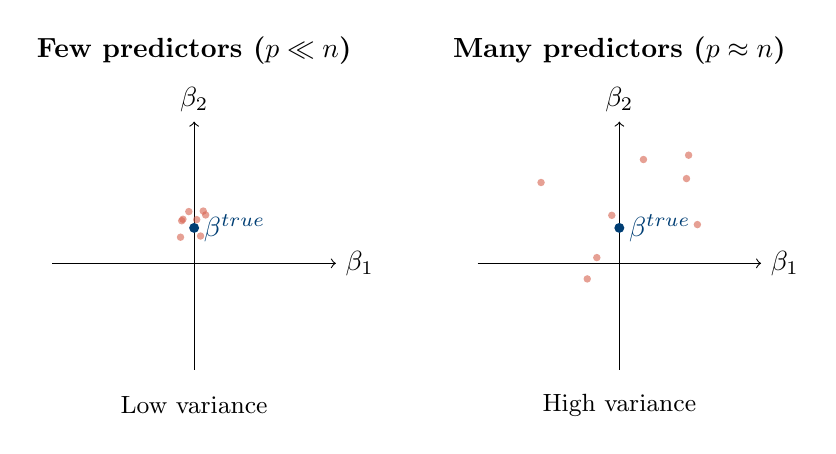
\begin{tikzpicture}[scale=0.9]
  % Left panel - low p
  \node at (-3, 3) {\textbf{Few predictors ($p \ll n$)}};
  \draw[->] (-5, 0) -- (-1, 0) node[right] {$\beta_1$};
  \draw[->] (-3, -1.5) -- (-3, 2) node[above] {$\beta_2$};
  \fill[ThemeBlue] (-3, 0.5) circle (2pt) node[right] {$\beta^{true}$};
  \foreach \i in {1,...,8} {
    \fill[AccentOrange, opacity=0.6] (-3 + 0.3*rand, 0.5 + 0.3*rand) circle (1.5pt);
  }
  \node at (-3, -2) {\small Low variance};
  
  % Right panel - high p
  \node at (3, 3) {\textbf{Many predictors ($p \approx n$)}};
  \draw[->] (1, 0) -- (5, 0) node[right] {$\beta_1$};
  \draw[->] (3, -1.5) -- (3, 2) node[above] {$\beta_2$};
  \fill[ThemeBlue] (3, 0.5) circle (2pt) node[right] {$\beta^{true}$};
  \foreach \i in {1,...,8} {
    \fill[AccentOrange, opacity=0.6] (3 + 1.2*rand, 0.5 + 1.2*rand) circle (1.5pt);
  }
  \node at (3, -2) {\small High variance};
\end{tikzpicture}
\end{center}

\vspace{0.5em}
Each orange point: $\widehat{\beta}^{OLS}$ from a different sample.

With many predictors, estimates are \highlight{scattered} around the true ${\color{ThemeBlue}\beta^{true}}$

\end{frame}

%----------------------------------------------------------------------------------------

\begin{frame}{The Overfitting Problem}

\textbf{In-sample:} Adding predictors always improves fit
\begin{itemize}
  \item $R^2$ increases (or stays the same)
  \item RSS decreases (or stays the same)
  \item Can achieve a perfect fit if $p = n$
\end{itemize}

\vspace{1em}
\textbf{Out-of-sample:} Performance often \emph{decreases}
\begin{itemize}
  \item Model fits noise, not signal
  \item Predictions on new data are poor
  \item May be worse than simple benchmarks
\end{itemize}

\vspace{1em}
\begin{block}{Reminder: The Golden Rule}
Always evaluate predictive performance \highlight{out-of-sample}.
\end{block}

\end{frame}

%----------------------------------------------------------------------------------------

\begin{frame}{The Solution --- Constrained Estimation}

\textbf{Key insight:} Accept some \highlight{bias} to reduce \highlight{variance}

\vspace{1em}
\textbf{Recall from Lecture 1:}
\[
\MSE(\widehat{\beta}) = \Bias(\widehat{\beta})^2 + \Var(\widehat{\beta})
\]

\vspace{0.5em}
\textbf{OLS:}
\begin{itemize}
  \item Zero bias (unbiased)
  \item High variance when $p$ is large
\end{itemize}

\vspace{0.5em}
\textbf{Regularized methods:}
\begin{itemize}
  \item Shrink coefficients toward zero
  \item Introduces bias, but substantially reduces variance
  \item Net effect: Lower total MSE
\end{itemize}

\vspace{1em}
\textbf{Intuition:} By being ``skeptical'' of extreme coefficient values, we avoid fitting noise in the training data.

\end{frame}

%----------------------------------------------------------------------------------------
\section{Ridge Regression}
%----------------------------------------------------------------------------------------

\begin{frame}{Ridge Regression --- The Idea}

\textbf{Problem with OLS:} Coefficients can be arbitrarily large

\vspace{1em}
\textbf{Solution:} Penalize large coefficients
\begin{itemize}
  \item Add a ``cost'' for coefficient magnitude
  \item Model must balance fit vs.\ coefficient size
  \item Large coefficients only if strongly supported by data
\end{itemize}

\vspace{1em}
\textbf{Intuition:} 
\begin{itemize}
  \item Without penalty: ``Use any coefficient values you want''
  \item With penalty: ``Large coefficients are expensive''
\end{itemize}

\end{frame}

%----------------------------------------------------------------------------------------

\begin{frame}{Ridge Regression --- Formulation}

\textbf{Penalized least squares:}
\[
\widehat{\beta}^{Ridge} = \argmin_\beta \left\{ \underbrace{\sum_{i=1}^n (y_i - x_i'\beta)^2}_{\text{RSS}} + \underbrace{\lambda \sum_{j=1}^p \beta_j^2}_{\text{Ridge Penalty}} \right\}
\]

\vspace{1em}
\textbf{The penalty term:}
\begin{itemize}
  \item $\sum_{j=1}^p \beta_j^2 = \|\beta\|_2^2$ is the squared $L_2$ norm
  \item Penalizes the sum of squared coefficients
  \item $\lambda \geq 0$ is a \highlight{penalty parameter} that needs to be tuned
\end{itemize}

\end{frame}

%----------------------------------------------------------------------------------------

\begin{frame}{The Role of $\lambda$}

The tuning parameter $\lambda$ controls the \highlight{strength of regularization}:

\vspace{1em}
\begin{itemize}
  \item $\lambda = 0$: No penalty $\Rightarrow$ recover OLS
  
  \vspace{0.5em}
  \item $\lambda \to \infty$: Infinite penalty $\Rightarrow$ all $\widehat{\beta}_j \to 0$
  
  \vspace{0.5em}
  \item Intermediate $\lambda$: Balance between fit and complexity
\end{itemize}

\vspace{1em}
\begin{block}{Key Point}
$\lambda$ is a \highlight{hyperparameter} --- not estimated from the objective function. We choose it separately (e.g., via cross-validation).
\end{block}

\end{frame}

%----------------------------------------------------------------------------------------

\begin{frame}{Equivalent Constrained Form}

Ridge regression can be written as a \textbf{constrained optimization}:
\[
\min_\beta \sum_{i=1}^n (y_i - x_i'\beta)^2 \qquad \text{subject to} \qquad \sum_{j=1}^p \beta_j^2 \leq t
\]

\vspace{1em}
\textbf{Interpretation:}
\begin{itemize}
  \item Minimize RSS subject to a ``budget'' on coefficients
  \item Budget $t$ corresponds to penalty $\lambda$ (one-to-one mapping)
  \item Smaller $t$ $\Leftrightarrow$ larger $\lambda$ $\Leftrightarrow$ more shrinkage
\end{itemize}

\vspace{1em}
\textbf{Geometric view:} Coefficients must lie within a sphere of radius $\sqrt{t}$.

\end{frame}

%----------------------------------------------------------------------------------------

\begin{frame}{Geometric Interpretation}

\begin{center}
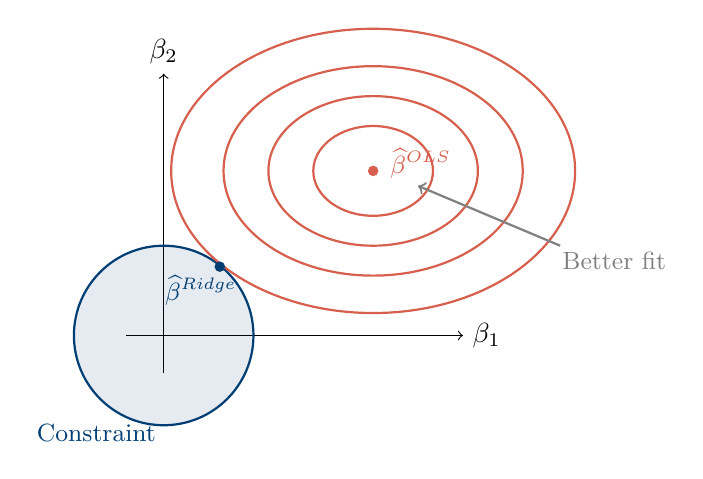
\begin{tikzpicture}[scale=0.95]
  % Axes
  \draw[->] (-0.5, 0) -- (4, 0) node[right] {$\beta_1$};
  \draw[->] (0, -0.5) -- (0, 3.5) node[above] {$\beta_2$};
  
  % Constraint region (circle)
  \draw[thick, ThemeBlue, fill=ThemeBlue, fill opacity=0.1] (0,0) circle (1.2);
  \node[ThemeBlue] at (-0.9, -1.3) {\small Constraint};
  
  % RSS contours (ellipses)
  \draw[AccentOrange, thick] (2.8, 2.2) ellipse (0.8 and 0.6);
  \draw[AccentOrange, thick] (2.8, 2.2) ellipse (1.4 and 1);
  \draw[AccentOrange, thick] (2.8, 2.2) ellipse (2 and 1.4);
  \draw[AccentOrange, thick] (2.8, 2.2) ellipse (2.7 and 1.9);
  
  % OLS solution
  \fill[AccentOrange] (2.8, 2.2) circle (2pt);
  \node[AccentOrange, right] at (2.9, 2.3) {\small $\widehat{\beta}^{OLS}$};
  
  % Ridge solution
  \fill[ThemeBlue] (0.75, 0.92) circle (2pt);
  \node[ThemeBlue, left] at (1.1, 0.6) {\small $\widehat{\beta}^{Ridge}$};
  
  % Arrow indicating "better fit"
  \draw[->, gray, thick] (5.3, 1.2) -- (3.4, 2.0);
  \node[gray, right] at (5.2, 1) {\small Better fit};
\end{tikzpicture}
\end{center}

\vspace{0.3em}
\begin{itemize}
  \item \textcolor{AccentOrange}{\textbf{Ellipses:}} Points with equal RSS (inner = better fit)
  \item \textcolor{ThemeBlue}{\textbf{Circle:}} Constraint region (coefficients must stay inside)
  \item \textbf{OLS:} $\widehat{\beta}^{OLS}$ best fit, ignoring the constraint
  \item \textbf{Ridge:} $\widehat{\beta}^{Ridge}$ best fit \emph{within} the constraint
\end{itemize}

\end{frame}

%----------------------------------------------------------------------------------------

\begin{frame}{Closed-Form Solution}

Ridge regression has an \textbf{analytical solution}:
\[
\widehat{\beta}^{Ridge} = (X'X + \lambda I)^{-1}X'y
\]

\vspace{0.5em}
Compare to OLS: $\widehat{\beta}^{OLS} = (X'X)^{-1}X'y$

\vspace{1em}
\textbf{Key insight:} Adding $\lambda I$ to $X'X$:
\begin{itemize}
  \item Ensures the matrix is always invertible (even if $p > n$)
  \item ``Stabilizes'' the estimation
  \item Larger $\lambda$ $\Rightarrow$ more shrinkage toward zero
\end{itemize}

\vspace{1em}
\textbf{Practical advantage:} Closed-form solution means fast computation, even with many predictors.

\end{frame}

%----------------------------------------------------------------------------------------

\begin{frame}{What Does Ridge Do? --- Shrinkage}

\textbf{Key properties:}
\begin{itemize}
  \item All coefficients are shrunk toward zero
  \item No coefficient is set exactly to zero (all predictors remain)
  \item Correlated predictors: Weight is shared more evenly across them
\end{itemize}

\vspace{1em}
\textbf{Intuition:} Ridge is ``skeptical'' of large coefficients --- requires strong evidence in the data to maintain them.

\vspace{1em}
\textbf{Financial interpretation:} 
\begin{itemize}
  \item Large coefficient = strong belief in predictability
  \item Shrinkage = disciplined skepticism
  \item Appropriate given concerns about data mining in finance
\end{itemize}

\end{frame}

%----------------------------------------------------------------------------------------

\begin{frame}{Bias-Variance Tradeoff for Ridge}

\textbf{Bias:} Ridge introduces bias
\begin{itemize}
  \item $\E[\widehat{\beta}^{Ridge}] \neq \beta$ (biased estimator)
  \item Coefficients are systematically shrunk toward zero
\end{itemize}

\vspace{1em}
\textbf{Variance:} Ridge reduces variance
\begin{itemize}
  \item $\Var(\widehat{\beta}^{Ridge}) < \Var(\widehat{\beta}^{OLS})$
  \item Shrinkage stabilizes estimates across different samples
\end{itemize}

\vspace{1em}
\textbf{MSE tradeoff:}
\begin{itemize}
  \item Small $\lambda$: Low bias, high variance (close to OLS)
  \item Large $\lambda$: High bias, low variance (close to zero)
  \item Optimal $\lambda$: Minimizes total MSE
\end{itemize}

\end{frame}

%----------------------------------------------------------------------------------------

\begin{frame}{MSE as a Function of $\lambda$}

\begin{center}
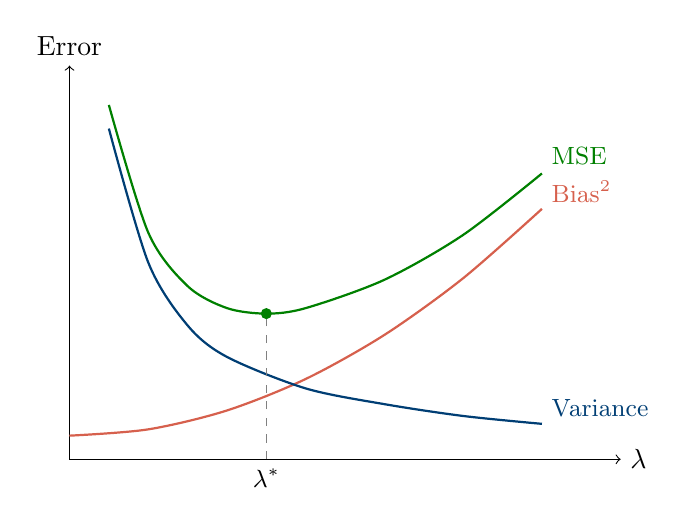
\begin{tikzpicture}[scale=1]
  % Axes
  \draw[->] (0, 0) -- (7, 0) node[right] {$\lambda$};
  \draw[->] (0, 0) -- (0, 5) node[above] {Error};
  
  % Bias squared (increasing) - manual coordinates
  \draw[thick, AccentOrange] plot[smooth] coordinates {
    (0, 0.3) (1, 0.38) (2, 0.62) (3, 1.02) (4, 1.58) (5, 2.3) (6, 3.18)
  };
  \node[AccentOrange, right] at (6, 3.4) {\small Bias$^2$};
  
  % Variance (decreasing) - manual coordinates
  \draw[thick, ThemeBlue] plot[smooth] coordinates {
    (0.5, 4.2) (1, 2.5) (1.5, 1.7) (2, 1.3) (3, 0.9) (4, 0.7) (5, 0.55) (6, 0.45)
  };
  \node[ThemeBlue, right] at (6, 0.65) {\small Variance};
  
  % MSE (U-shaped) - manual coordinates
  \draw[thick, AccentGreen] plot[smooth] coordinates {
    (0.5, 4.5) (1, 2.88) (1.5, 2.2) (2, 1.92) (2.5, 1.85) (3, 1.92) (4, 2.28) (5, 2.85) (6, 3.63)
  };
  \node[AccentGreen, right] at (6, 3.85) {\small MSE};
  
  % Optimal lambda
  \draw[dashed, gray] (2.5, 0) -- (2.5, 1.85);
  \node[below] at (2.5, 0) {\small $\lambda^*$};
  \fill[AccentGreen] (2.5, 1.85) circle (2pt);
\end{tikzpicture}
\end{center}

\vspace{0.5em}
Optimal $\lambda^*$ balances bias and variance to minimize total MSE.

\end{frame}

%----------------------------------------------------------------------------------------

\begin{frame}{Important: Feature Scaling}

\textbf{Problem:} Ridge penalty depends on coefficient magnitude
\[
\text{Penalty} = \lambda \sum_{j=1}^p \beta_j^2
\]

If predictors are on different scales (e.g., dollars vs.\ millions):
\begin{itemize}
  \item Coefficients $\beta_j$ have different magnitudes
  \item Penalty affects them unequally
\end{itemize}

\vspace{1em}
\textbf{Solution:} \highlight{Standardize} each feature before estimation
\[
\tilde{x}_{ij} = \frac{x_{ij} - \bar{x}_j}{s_j}
\]
\begin{itemize}
  \item Each feature has mean zero, standard deviation one
  \item Coefficients become comparable
  \item In sklearn: \texttt{StandardScaler()} handles this automatically
\end{itemize}

\end{frame}

%----------------------------------------------------------------------------------------
\section{Lasso Regression}
%----------------------------------------------------------------------------------------

\begin{frame}{Limitation of Ridge}

\textbf{Ridge regression:}
\begin{itemize}
  \item Shrinks all coefficients toward zero
  \item But: Never sets coefficients \emph{exactly} to zero
  \item All $p$ predictors remain in the model
\end{itemize}

\vspace{1em}
\textbf{When is this a problem?}
\begin{itemize}
  \item Many irrelevant predictors (want to exclude them)
  \item Desire for interpretability (which variables matter?)
  \item Sparse models may generalize better out-of-sample
\end{itemize}

\vspace{1em}
\textbf{Want:} A method that performs \highlight{variable selection} automatically.

\end{frame}

%----------------------------------------------------------------------------------------

\begin{frame}{Lasso --- Formulation}

\textbf{Least Absolute Shrinkage and Selection Operator} (Tibshirani, 1996):
\[
\widehat{\beta}^{Lasso} = \argmin_\beta \left\{ \sum_{i=1}^n (y_i - x_i'\beta)^2 + \lambda \sum_{j=1}^p |\beta_j| \right\}
\]

\vspace{1em}
\textbf{Key difference from Ridge:}
\begin{itemize}
  \item Ridge: $L_2$ penalty $\sum_j \beta_j^2$ (squared coefficients)
  \item Lasso: $L_1$ penalty $\sum_j |\beta_j|$ (absolute values)
\end{itemize}

\vspace{1em}
\textbf{Crucial property:} Lasso produces \highlight{sparse} solutions --- some $\widehat{\beta}_j = 0$ exactly.

\end{frame}

%----------------------------------------------------------------------------------------

\begin{frame}{The Key Difference: Ridge vs. Lasso Penalties}

\begin{center}
\begin{tabular}{p{0.45\textwidth} p{0.45\textwidth}}
\textbf{Ridge Regression (L2)} & \textbf{Lasso Regression (L1)} \\
\cmidrule(r){1-1}\cmidrule(l){2-2}
Penalizes \highlight{squares}: $\beta^2$ & Penalizes \highlight{absolute values}: $|\beta|$ \\
& \\
Shrinks coefficients proportionally & Pushes coefficients toward zero \\
\highlight{Never becomes exactly zero} & \highlight{Can become exactly zero} \\
\end{tabular}
\end{center}

\vspace{1em}

\textbf{Visualizing the Penalty Effect:}

\begin{center}
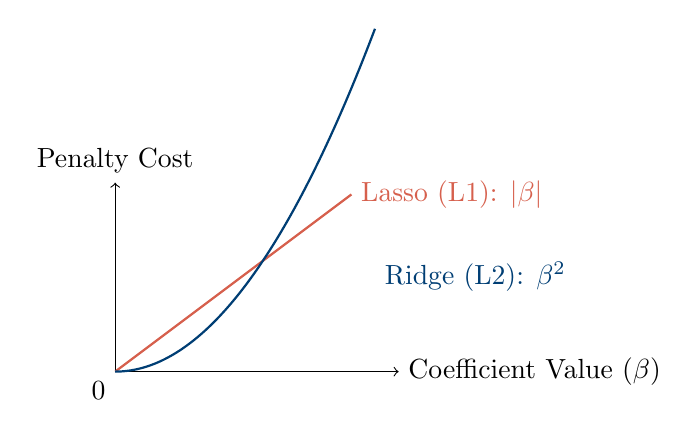
\begin{tikzpicture}[scale=0.6]
% Axes
\draw[->] (0,0) -- (6,0) node[right] {Coefficient Value ($\beta$)};
\draw[->] (0,0) -- (0,4) node[above] {Penalty Cost};

% L1 penalty (Lasso)
\draw[thick, AccentOrange] (0,0) -- (5,3.75);
\node[AccentOrange, right] at (5,3.75) {Lasso (L1): $|\beta|$};

% L2 penalty (Ridge) - parabola
\draw[thick, ThemeBlue] plot [domain=0:2.2, samples=100] (\x*2.5, {(\x*\x)*1.5});
\node[ThemeBlue, right] at (5.5,2) {Ridge (L2): $\beta^2$};

% Zero point
\node at (0,0) [below left] {0};
\end{tikzpicture}
\end{center}

\vspace{0.5em}

\textbf{The Analogy:}
\begin{itemize}
  \item \textcolor{ThemeBlue}{\textbf{Ridge}} is like a rubber band - hard to pull all the way to zero
  \item \textcolor{AccentOrange}{\textbf{Lasso}} has a spring-loaded latch at zero - weak coefficients snap to zero
\end{itemize}

\end{frame}


\begin{frame}{How Lasso Works: The ``Soft Thresholding'' Rule}

\textbf{A Simple Decision Rule:}

Lasso asks each variable: \textit{``Is your signal strong enough to survive the penalty?''}

\vspace{1em}

For each coefficient:
\begin{enumerate}
  \item Start with the regular model coefficient ($\widehat{\beta}_{OLS}$)
  \item Subtract the Lasso penalty ($\lambda$)
  \item Apply the decision rule:
    \begin{itemize}
      \item If result is \textbf{positive} $\rightarrow$ keep it
      \item If result is \textbf{negative} $\rightarrow$ set to \textbf{zero}
    \end{itemize}
\end{enumerate}

\vspace{1em}

\textbf{Example:} (with penalty $\lambda = 0.5$)

\begin{center}
\begin{tabular}{llll}
 & \textbf{Step 1:} & \textbf{Step 2:} & \textbf{Step 3:} \\
 & $\widehat{\beta}_{OLS}$ & Subtract $\lambda$ & Final Decision \\
\cmidrule(r){1-1}\cmidrule(lr){2-2}\cmidrule(lr){3-3}\cmidrule(l){4-4}
Variable A & 1.2 & 1.2 - 0.5 = 0.7 & \textbf{Kept} (0.7) \\
Variable B & 0.4 & 0.4 - 0.5 = -0.1 & \textbf{Set to ZERO} \\
Variable C & -0.8 & |-0.8| - 0.5 = 0.3 & \textbf{Kept} (-0.3) \\
\end{tabular}
\end{center}

\end{frame}

%----------------------------------------------------------------------------------------

%----------------------------------------------------------------------------------------

%----------------------------------------------------------------------------------------

\begin{frame}{Shrinkage Comparison: Ridge vs.\ Lasso}

\begin{center}
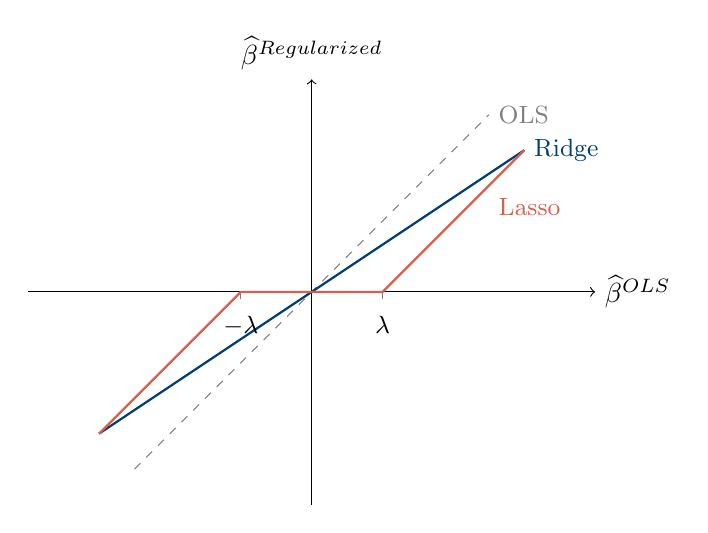
\begin{tikzpicture}[scale=0.9]
  % Axes
  \draw[->] (-4, 0) -- (4, 0) node[right] {$\widehat{\beta}^{OLS}$};
  \draw[->] (0, -3) -- (0, 3) node[above] {$\widehat{\beta}^{Regularized}$};
  
  % 45-degree line (OLS)
  \draw[gray, dashed] (-2.5, -2.5) -- (2.5, 2.5);
  \node[gray, right] at (2.5, 2.5) {\small OLS};
  
  % Ridge (proportional shrinkage)
  \draw[thick, ThemeBlue] (-3, -2) -- (3, 2);
  \node[ThemeBlue, right] at (3, 2) {\small Ridge};
  
  % Lasso (soft thresholding)
  \draw[thick, AccentOrange] (-3, -2) -- (-1, 0) -- (1, 0) -- (3, 2);
  \node[AccentOrange, right] at (2.5, 1.2) {\small Lasso};
  
  % Lambda markers
  \draw[dashed, gray] (1, -0.1) -- (1, 0.1);
  \draw[dashed, gray] (-1, -0.1) -- (-1, 0.1);
  \node[below] at (1, -0.2) {\small $\lambda$};
  \node[below] at (-1, -0.2) {\small $-\lambda$};
\end{tikzpicture}
\end{center}

\vspace{0.5em}
Ridge: Proportional shrinkage (all coefficients reduced). \\
Lasso: Soft thresholding (small coefficients set to zero).

\end{frame}

%----------------------------------------------------------------------------------------

\begin{frame}{Lasso --- No Closed-Form Solution}

\textbf{General case:} No analytical solution for Lasso

\vspace{1em}
\textbf{Why?}
\begin{itemize}
  \item The $L_1$ penalty $|\beta_j|$ is not differentiable at zero
  \item Cannot set derivative to zero and solve
\end{itemize}

\vspace{1em}
\textbf{Solution:} Iterative optimization algorithms
\begin{itemize}
  \item Coordinate descent: Update one $\beta_j$ at a time
  \item Very efficient implementations exist
  \item sklearn uses fast coordinate descent
\end{itemize}

\vspace{1em}
\textbf{Practical implementation:} Slightly slower than Ridge, but still fast.

\end{frame}

%----------------------------------------------------------------------------------------

\begin{frame}{Lasso --- Properties}

\textbf{Advantages:}
\begin{itemize}
  \item Automatic variable selection (sparse solutions)
  \item Interpretability: Identifies ``important'' predictors
  \item Can handle $p > n$ (selects at most $n$ variables)
\end{itemize}

\vspace{1em}
\textbf{Limitations:}
\begin{itemize}
  \item With correlated predictors: Selects one arbitrarily
  \item Can be unstable: Different samples $\Rightarrow$ different selections
  \item At most $\min(n, p)$ non-zero coefficients
\end{itemize}

\vspace{1em}
\textbf{Next:} what to do when correlation matters but we still want to do variable selection.

\end{frame}

%----------------------------------------------------------------------------------------
\section{Elastic Net}
%----------------------------------------------------------------------------------------

\begin{frame}{Combining Ridge and Lasso}

\textbf{Ridge:}
\begin{itemize}
  \item[$+$] Handles correlated predictors well
  \item[$+$] Stable estimates
  \item[$-$] No variable selection (keeps all predictors)
\end{itemize}

\vspace{0.5em}
\textbf{Lasso:}
\begin{itemize}
  \item[$+$] Automatic variable selection
  \item[$+$] Sparse, interpretable models
  \item[$-$] Unstable with correlated predictors
\end{itemize}

\vspace{1em}
\textbf{Elastic Net:} Combine both penalties to get the best of both worlds.

\end{frame}

%----------------------------------------------------------------------------------------

\begin{frame}{Elastic Net --- Formulation}

\textbf{Zou \& Hastie (2005):}
\[
\widehat{\beta}^{EN} = \argmin_\beta \left\{ \sum_{i=1}^n (y_i - x_i'\beta)^2 + \lambda \left[ \alpha \sum_{j=1}^p |\beta_j| + (1-\alpha) \sum_{j=1}^p \beta_j^2 \right] \right\}
\]

\vspace{1em}
\textbf{Two hyperparameters:}
\begin{itemize}
  \item $\lambda \geq 0$: Overall penalty strength
  \item $\alpha \in [0, 1]$: Mixing parameter
  \begin{itemize}
    \item $\alpha = 1$: Pure Lasso
    \item $\alpha = 0$: Pure Ridge
    \item $\alpha \in (0,1)$: Combination
  \end{itemize}
\end{itemize}

\end{frame}

%----------------------------------------------------------------------------------------

\begin{frame}{Elastic Net --- Properties}

\textbf{Inherits advantages of both methods:}

\vspace{1em}
From Lasso ($L_1$ component):
\begin{itemize}
  \item Sparse solutions (variable selection)
  \item Can set coefficients exactly to zero
\end{itemize}

\vspace{0.5em}
From Ridge ($L_2$ component):
\begin{itemize}
  \item \highlight{Grouping effect}: Correlated predictors selected together
  \item More stable than pure Lasso
  \item Can select more than $n$ variables
\end{itemize}

\vspace{1em}
\textbf{In practice:} Often the best choice for high-dimensional problems.

\end{frame}

%----------------------------------------------------------------------------------------

%----------------------------------------------------------------------------------------

\begin{frame}{Method Comparison}

\begin{center}
\begin{tabular}{lcccc}
\toprule
\textbf{Method} & \textbf{Penalty} & \textbf{Sparse?} & \textbf{Closed-form?} & \textbf{Correlation} \\
\midrule
OLS & None & No & Yes & Poor \\
Ridge & $L_2$ & No & Yes & Good \\
Lasso & $L_1$ & Yes & No & Poor \\
Elastic Net & $L_1 + L_2$ & Yes & No & Good \\
\bottomrule
\end{tabular}
\end{center}

\vspace{1em}
\textbf{Guidance:}
\begin{itemize}
  \item Few predictors, low correlation $\Rightarrow$ OLS may suffice
  \item Many correlated predictors $\Rightarrow$ Ridge or Elastic Net
  \item Want variable selection $\Rightarrow$ Lasso or Elastic Net
  \item High-dimensional, correlated $\Rightarrow$ Elastic Net
\end{itemize}

\end{frame}

%----------------------------------------------------------------------------------------

\begin{frame}{Recap: Key Equations}

\textbf{OLS:}
\[
\widehat{\beta}^{OLS} = (X'X)^{-1}X'y
\]

\vspace{0.5em}
\textbf{Ridge:}
\[
\widehat{\beta}^{Ridge} = (X'X + \lambda I)^{-1}X'y
\]

\vspace{0.5em}
\textbf{Lasso:}
\[
\widehat{\beta}^{Lasso} = \argmin_\beta \left\{ \sum_{i=1}^n (y_i - x_i'\beta)^2 + \lambda \sum_{j=1}^p |\beta_j| \right\}
\]

\vspace{0.5em}
\textbf{Elastic Net:}
\[
\widehat{\beta}^{EN} = \argmin_\beta \left\{ \sum_{i=1}^n (y_i - x_i'\beta)^2 + \lambda \left[ \alpha \sum_{j=1}^p |\beta_j| + (1-\alpha) \sum_{j=1}^p \beta_j^2 \right] \right\}
\]

\end{frame}

%----------------------------------------------------------------------------------------

%======================== PART II CONTENT ========================

%----------------------------------------------------------------------------------------
\section{Selecting $\lambda$ in Penalized Regressions}
%----------------------------------------------------------------------------------------

\begin{frame}{The Critical Question}

Remember: Ridge, Lasso, Elastic Net all depend on $\lambda$ (and $\alpha$).

\vspace{1em}
\textbf{How do we choose these hyperparameters?}

\vspace{0.5em}
Cannot use training sample:
\begin{itemize}
  \item Training error always decreases with less regularization
  \item Would select $\lambda = 0$ (back to OLS)
  \item Overfits to training data
\end{itemize}

\vspace{1em}
\textbf{Need:} A proxy for the  \highlight{out-of-sample} performance of the model. 

\end{frame}

%----------------------------------------------------------------------------------------

\begin{frame}{Cross-Validation: Review}
  K-\textbf{Fold Cross-Validation}
  
  \begin{center}
  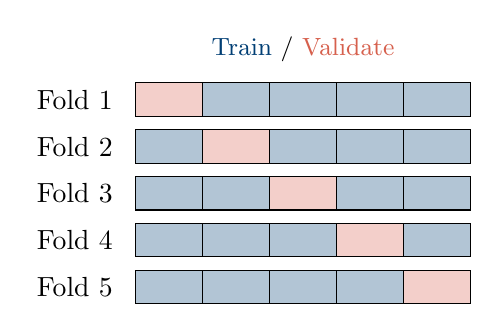
\begin{tikzpicture}[scale=0.85]
    \foreach \i in {1,...,5} {
      \foreach \j in {1,...,5} {
        \ifnum\j=\i
          \draw[fill=AccentOrange!30] (\j-1, -\i*0.7) rectangle (\j, -\i*0.7+0.5);
        \else
          \draw[fill=ThemeBlue!30] (\j-1, -\i*0.7) rectangle (\j, -\i*0.7+0.5);
        \fi
      }
      \node[left] at (-0.2, -\i*0.7+0.25) {Fold \i};
    }
    \node at (2.5, 0.3) {\small \textcolor{ThemeBlue}{Train} / \textcolor{AccentOrange}{Validate}};
  \end{tikzpicture}
  \end{center}
  
  \textbf{Procedure:}
  \begin{enumerate}
    \item Split data into K equal parts (``folds'')
    \item For each fold: train on other K-1 folds, validate the prediction error on this fold
    \item Average the K prediction errors
  \end{enumerate}
  
  \textbf{Common choice:} K = 5 or K = 10
\end{frame}


%----------------------------------------------------------------------------------------

\begin{frame}{Problem: Time Series Structure}
\textbf{Standard CV:} Observations are exchangeable (order does not matter).
  
\begin{center}
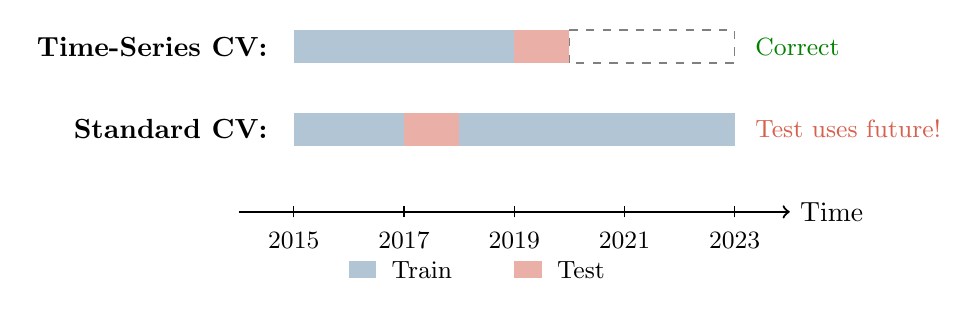
\begin{tikzpicture}[scale=0.7]
  % Timeline
  \draw[thick, ->] (0, 0) -- (10, 0) node[right] {Time};
  
  % Year markers
  \foreach \x/\year in {1/2015, 3/2017, 5/2019, 7/2021, 9/2023} {
    \draw (\x, -0.1) -- (\x, 0.1);
    \node[below] at (\x, -0.2) {\small \year};
  }
  
  % Standard CV (wrong)
  \node[left] at (0.7, 1.5) {\textbf{Standard CV:}};
  \fill[ThemeBlue, opacity=0.3] (1, 1.2) rectangle (3, 1.8);
  \fill[AccentOrange, opacity=0.5] (3, 1.2) rectangle (4, 1.8);
  \fill[ThemeBlue, opacity=0.3] (4, 1.2) rectangle (9, 1.8);
  \node[right] at (9.2, 1.5) {\small \textcolor{AccentOrange}{Test uses future!}};
  
  % Time series CV (correct)
  \node[left] at (0.7, 3) {\textbf{Time-Series CV:}};
  \fill[ThemeBlue, opacity=0.3] (1, 2.7) rectangle (5, 3.3);
  \fill[AccentOrange, opacity=0.5] (5, 2.7) rectangle (6, 3.3);
  \fill[white] (6, 2.7) rectangle (9, 3.3);
  \draw[dashed, gray] (6, 2.7) rectangle (9, 3.3);
  \node[right] at (9.2, 3) {\small \textcolor{AccentGreen}{Correct}};
  
  % Legend
  \fill[ThemeBlue, opacity=0.3] (2, -1.2) rectangle (2.5, -0.9);
  \node[right] at (2.6, -1.05) {\small Train};
  \fill[AccentOrange, opacity=0.5] (5, -1.2) rectangle (5.5, -0.9);
  \node[right] at (5.6, -1.05) {\small Test};
\end{tikzpicture}
\end{center}

\textbf{Time series reality:}
\begin{itemize}
  \item Observations are ordered in time
  \item Cannot use future data to predict past
\end{itemize}

\vspace{0.5em}
\textbf{Random splits create \highlight{look-ahead bias}:}
\begin{itemize}
  \item Model trained on 2015--2020 data
  \item Tested on 2018 data (performance is biased!)
\end{itemize}


\end{frame}

%----------------------------------------------------------------------------------------

\begin{frame}{Time-Series Cross-Validation}

\textbf{Key principle:} Always train on past, test on future.
\vspace{-0.1in}
\begin{center}
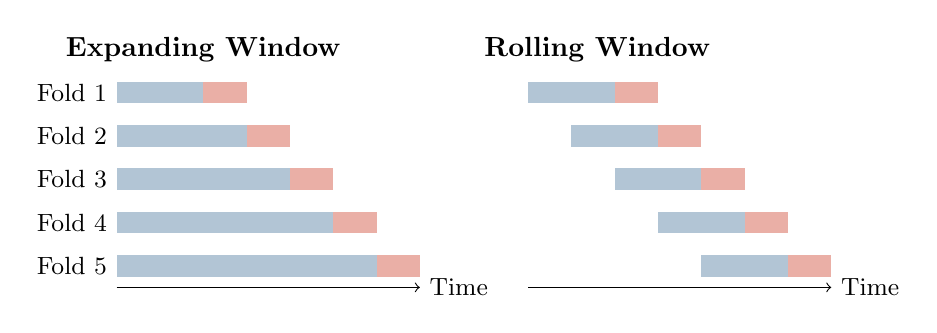
\begin{tikzpicture}[scale=0.55]
  % Expanding window
  \node at (1.5, 5) {\textbf{Expanding Window}};
  
  \foreach \i in {1,...,5} {
    \pgfmathsetmacro{\trainend}{1 + \i}
    \pgfmathsetmacro{\teststart}{\trainend}
    \pgfmathsetmacro{\testend}{\trainend + 0.5}
    \pgfmathsetmacro{\ypos}{5 - \i}
    
    % Train
    \fill[ThemeBlue, opacity=0.3] (-0.5, \ypos - 0.25) rectangle (\trainend - 0.5, \ypos + 0.25);
    % Test
    \fill[AccentOrange, opacity=0.5] (\teststart - 0.5, \ypos - 0.25) rectangle (\testend, \ypos + 0.25);
    % Label
    \node[left] at (-0.5, \ypos) {\small Fold \i};
  }
  
  % Timeline
  \draw[->] (-0.5, -0.5) -- (6.5, -0.5);
  \node[right] at (6.5, -0.5) {\small Time};
  
  % Rolling window (right side)
  \node at (10.6, 5) {\textbf{Rolling Window}};
  
  \foreach \i in {1,...,5} {
    \pgfmathsetmacro{\trainstart}{\i}
    \pgfmathsetmacro{\trainend}{\i + 2}
    \pgfmathsetmacro{\teststart}{\trainend}
    \pgfmathsetmacro{\testend}{\trainend + 1}
    \pgfmathsetmacro{\ypos}{5 - \i}
    
    % Train
    \fill[ThemeBlue, opacity=0.3] (9 + \trainstart - 1, \ypos - 0.25) rectangle (9 + \trainend - 1, \ypos + 0.25);
    % Test
    \fill[AccentOrange, opacity=0.5] (9 + \teststart - 1, \ypos - 0.25) rectangle (9 + \testend - 1, \ypos + 0.25);
  }
  
  % Timeline
  \draw[->] (9, -0.5) -- (16, -0.5);
  \node[right] at (16, -0.5) {\small Time};
\end{tikzpicture}
\end{center}

\textcolor{ThemeBlue}{$\blacksquare$} Training set \quad \textcolor{AccentOrange}{$\blacksquare$} Test set

\vspace{1em}
\highlight{Both respect temporal ordering} --- no look-ahead bias.
\begin{itemize}
    \item \textbf{Expanding window:} More data as we move forward; assumes stable relationships
    \item  \textbf{Rolling window:} Older data dropped as new data added; adapts to regime changes
\end{itemize}
\end{frame}

%----------------------------------------------------------------------------------------

\begin{frame}{Choosing $\lambda$: Procedure}
\textbf{Step 1:} Define a grid of candidate $\lambda$ values
\begin{itemize}
  \item Spaced on log scale (factors of 10): $\lambda \in \{0.001, 0.01, 0.1, 1, 10, 100\}$
\end{itemize}

\vspace{0.5em}
\textbf{Step 2:} For each $\lambda$, compute time-series CV error
\begin{itemize}
  \item Use 5-fold time-series CV on training data
  \item For each fold $k$: calculate prediction error $\text{MSE}_k(\lambda)$
  \item Average across folds: $\overline{\text{CV}}(\lambda) = \frac{1}{5}\sum_{k=1}^5 \text{MSE}_k(\lambda)$
  \item \highlight{Standard error}: $\text{SE}(\lambda) = \sqrt{\frac{1}{5}\sum_{k=1}^5 (\text{MSE}_k(\lambda) - \overline{\text{CV}}(\lambda))^2}$
\end{itemize}

\vspace{0.5em}
\textbf{Step 3:} Plot CV error vs.\ $\lambda$ with error bars

\vspace{0.5em}
\textbf{Step 4:} Select optimal $\lambda$
\begin{itemize}
  \item Option A: $\lambda_{\min}$ that minimizes $\overline{\text{CV}}(\lambda)$
  \item Option B: Largest $\lambda$ where $\overline{\text{CV}}(\lambda) \leq \overline{\text{CV}}(\lambda_{\min}) + \text{SE}(\lambda_{\min})$
\end{itemize}
\end{frame}

%----------------------------------------------------------------------------------------

\begin{frame}{Understanding the Standard Error in CV}
\textbf{Why do we need the standard error?}

\vspace{0.5em}
\begin{itemize}
  \item CV error is computed on \highlight{5 different validation folds}
  \item Each fold gives a slightly different error estimate
  \item The \highlight{standard error measures variability} across folds
\end{itemize}

\vspace{1em}
\textbf{Example for Ridge with $\lambda = 10$:}

\begin{table}[h]
\centering
\small
\begin{tabular}{cc}
\toprule
\textbf{Fold} & \textbf{MSE} \\
\midrule
Fold 1 & 0.0042 \\
Fold 2 & 0.0038 \\
Fold 3 & 0.0045 \\
Fold 4 & 0.0041 \\
Fold 5 & 0.0039 \\
\midrule
Mean & 0.0041 \\
Std. Dev. & 0.00026 \\
\textbf{Std. Error (SE)} & \textbf{0.00012} \\
\bottomrule
\end{tabular}
\end{table}

\vspace{0.5em}
{\small Note: SE = Std. Dev. / $\sqrt{5}$ measures uncertainty in mean CV error}
\end{frame}

%----------------------------------------------------------------------------------------

\begin{frame}{Choosing $\lambda$: The 1-Standard-Error Rule}
\begin{center}
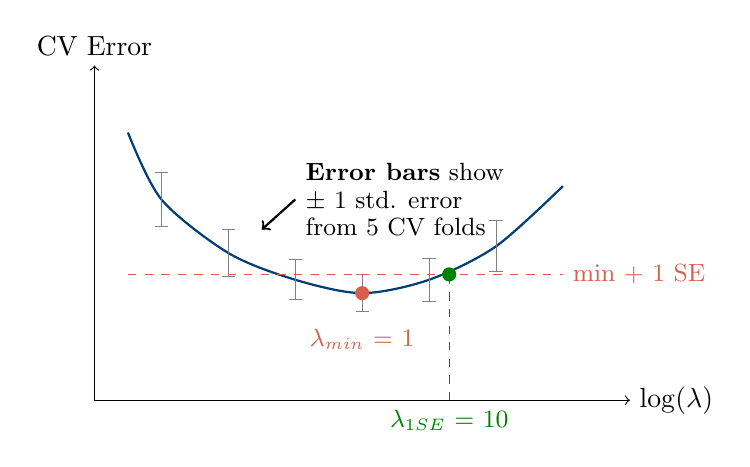
\begin{tikzpicture}[scale=0.85]
  % Axes
  \draw[->] (0, 0) -- (8, 0) node[right] {$\log(\lambda)$};
  \draw[->] (0, 0) -- (0, 5) node[above] {CV Error};
  
  % CV curve
  \draw[thick, ThemeBlue] plot[smooth] coordinates {
    (0.5, 4) (1, 3) (2, 2.2) (3, 1.8) (4, 1.6) (5, 1.8) (6, 2.3) (7, 3.2)
  };
  
  % Error bars (now labeled)
  \foreach \x/\y/\err in {1/3/0.4, 2/2.2/0.35, 3/1.8/0.3, 4/1.6/0.28, 5/1.8/0.32, 6/2.3/0.38} {
    \draw[gray] (\x, \y - \err) -- (\x, \y + \err);
    \draw[gray] (\x - 0.1, \y - \err) -- (\x + 0.1, \y - \err);
    \draw[gray] (\x - 0.1, \y + \err) -- (\x + 0.1, \y + \err);
  }
  
  % Add arrow pointing to error bar
  \draw[<-, thick] (2.5, 2.55) -- (3, 3) node[right, align=left] {\small \textbf{Error bars} show\\[-2pt] \small $\pm$ 1 std. error\\[-2pt] \small from 5 CV folds};
  
  % Minimum
  \fill[AccentOrange] (4, 1.6) circle (3pt);
  \node[AccentOrange, below] at (4, 1.2) {\small $\lambda_{min}$ = 1};
  
  % 1-SE line
  \draw[dashed, AccentOrange] (0.5, 1.88) -- (7, 1.88);
  \node[AccentOrange, right] at (7, 1.88) {\small min + 1 SE};
  
  % 1-SE lambda
  \fill[AccentGreen] (5.3, 1.88) circle (3pt);
  \draw[dashed, AccentGreen] (5.3, 0) -- (5.3, 1.88);
  \node[AccentGreen, below] at (5.3, 0) {\small $\lambda_{1SE}$ = 10};
\end{tikzpicture}
\end{center}

\vspace{-0.3em}
{\small
\textbf{1-SE rule intuition:} If $\lambda = 10$ performs within 1 SE of $\lambda = 1$, the difference could be \highlight{just noise from CV sampling}. Choose the simpler model ($\lambda = 10$ = more regularization).
}
\end{frame}

%----------------------------------------------------------------------------------------

\begin{frame}{Why Use the 1-SE Rule?}

\textbf{Motivation:} Protect against overfitting to the validation set

\vspace{1em}
\begin{columns}[T]
\column{0.48\textwidth}
\textbf{$\lambda_{\min}$ (minimum CV error):}
\begin{itemize}
  \item[$+$] Best on validation data
  \item[$-$] May overfit to noise in validation folds
  \item[$-$] Less regularization
  \item[$-$] More complex model
\end{itemize}

\column{0.48\textwidth}
\textbf{$\lambda_{1SE}$ (1-SE rule):}
\begin{itemize}
  \item[$+$] More conservative
  \item[$+$] Simpler model (more shrinkage)
  \item[$+$] Often better on true test data
  \item[$-$] Slightly worse on validation
\end{itemize}
\end{columns}

\vspace{1em}
\begin{block}{Practical Advice}
\begin{itemize}
  \item \textbf{Default:} Use $\lambda_{1SE}$ for most applications
  \item \textbf{Alternative:} Use $\lambda_{\min}$ if you have lots of data and computational budget for extensive CV
  \item \textbf{Both:} Try both and compare on final test set
\end{itemize}
\end{block}
\end{frame}

%----------------------------------------------------------------------------------------

\begin{frame}{Example: Ridge Regression CV Results}

\textbf{Suppose we get these results from 5-fold time-series CV:}

\begin{table}[h]
\centering
\small
\begin{tabular}{cccc}
\toprule
\textbf{$\lambda$} & \textbf{Mean CV Error} & \textbf{Std Error} & \textbf{Min + 1 SE} \\
\midrule
0.001 & 0.0052 & 0.00018 & --- \\
0.01  & 0.0048 & 0.00016 & --- \\
0.1   & 0.0044 & 0.00015 & --- \\
1     & \highlightgreen{0.0041} & 0.00012 & 0.0041 + 0.00012 = \highlightgreen{0.00422} \\
10    & 0.0042 & 0.00013 & --- \\
100   & 0.0046 & 0.00014 & --- \\
\bottomrule
\end{tabular}
\end{table}

\vspace{0.5em}
\begin{itemize}
  \item \textbf{$\lambda_{\min}$:} $\lambda = 1$ has lowest CV error (0.0041)
  \item \textbf{1-SE threshold:} 0.0041 + 0.00012 = 0.00422
  \item \textbf{$\lambda_{1SE}$:} $\lambda = 10$ has CV error 0.0042 $<$ 0.00422 $\checkmark$
  \item Higher $\lambda$ (100) exceeds threshold, so choose $\lambda = 10$
\end{itemize}

\vspace{0.5em}
\textbf{Interpretation:} $\lambda = 10$ is statistically indistinguishable from $\lambda = 1$, but simpler (more regularization), so we prefer it.
\end{frame}

%----------------------------------------------------------------------------------------


%----------------------------------------------------------------------------------------
\section{Application 1: Market Timing}
%----------------------------------------------------------------------------------------

\begin{frame}{The Equity Premium Prediction Problem}

\textbf{Central question:} Can we predict the stock market?

\vspace{1em}
\textbf{If YES:}
\begin{itemize}
  \item Time the market (shift allocation between stocks and bonds)
  \item Significant economic value
\end{itemize}

\vspace{0.5em}
\textbf{If NO:}
\begin{itemize}
  \item Buy and hold is optimal
  \item Active timing destroys value (transaction costs)
\end{itemize}

\vspace{1em}
\textbf{Academic debate:} Decades of research, no consensus.

\end{frame}

%----------------------------------------------------------------------------------------

\begin{frame}{The Prediction Model}

\textbf{Time-series regression:}
\[
r_{m,t+1} = \alpha + x_t'\boldsymbol{\beta} + \epsilon_{t+1}
\]
\textbf{Variables:}
\begin{itemize}
  \item $r_{m,t+1}$: Market excess return in month $t+1$
  \item $x_t$: Vector of predictor variables known at time $t$
  \item $\boldsymbol{\beta}$: Coefficients capturing predictive relationships
\end{itemize}

\vspace{1em}
\textbf{Goal:} Forecast $r_{m,t+1}$ using information available at $t$.

\vspace{1em}

\textbf{Classical predictors:} $\sim$15--20 variables commonly used in the literature
\begin{itemize}
  \item Valuation ratios: Dividend-price ratio (D/P), Earnings-price ratio (E/P), Book-to-market ratio (B/M)
  \item Interest rates: Treasury bill rate, Term spread (long minus short rates), Default spread (BAA minus AAA yields)
  \item Other: Stock variance, Inflation, Net equity expansion
\end{itemize}

% \vspace{0.5em}
% \textbf{Interest rates:}
% \begin{itemize}
%   \item 
%   \item 
%   \item 
% \end{itemize}

% \vspace{0.5em}
% \textbf{Other:}
% \begin{itemize}
%   \item Stock variance
%   \item Inflation
%   \item Net equity expansion
% \end{itemize}

% \vspace{0.5em}
% .

% \textbf{Challenge:} Low signal-to-noise ratio in returns.

\end{frame}

%----------------------------------------------------------------------------------------

\begin{frame}{The Benchmark: Historical Mean}

\textbf{Simplest possible forecast:}
\[
\widehat{r}_{t+1} = \bar{r}_t = \frac{1}{t} \sum_{s=1}^{t} r_s
\]

\vspace{0.5em}
Expanding-window average of past returns (Campbell and Thompson 2008). 

\vspace{1em}
\textbf{Economic underpinning:}
\begin{itemize}
  \item No predictability
  \item Constant expected return
  \item Ignores all predictor variables
\end{itemize}

\vspace{1em}
\begin{block}{Key Insight}
This naive benchmark is \highlight{surprisingly hard to beat} out-of-sample.
\end{block}

\end{frame}

%----------------------------------------------------------------------------------------

\begin{frame}{Measuring Forecast Quality: $R^2_{OS}$}

\textbf{Out-of-sample $R^2$:}
\[
R^2_{OS} = 1 - \frac{\sum_{t=t_0}^{T-1}(r_{t+1} - \widehat{r}_{t+1})^2}{\sum_{t=t_0}^{T-1}(r_{t+1} - \bar{r}_{t})^2}
\]
\textbf{Interpretation:}
\begin{itemize}
  \item $R^2_{OS} > 0$: Model beats the historical mean
  \item $R^2_{OS} = 0$: Model equals the historical mean
  \item $R^2_{OS} < 0$: Model is \emph{worse} than the mean
\end{itemize}

\vspace{1em}
\textbf{Key difference from in-sample $R^2$:}
\begin{itemize}
  \item In-sample $R^2 \geq 0$ always
  \item Out-of-sample $R^2_{OS}$ can be negative!
\end{itemize}

\end{frame}

%----------------------------------------------------------------------------------------

\begin{frame}{Goyal \& Welch (2008): Original Findings}

\textbf{Comprehensive study} of equity premium prediction.

\vspace{1em}
\textbf{Methodology:}
\begin{itemize}
  \item Test all major predictors from the literature
  \item Proper out-of-sample evaluation
  \item Expanding window estimation
\end{itemize}

\vspace{1em}
\textbf{Results:}
\begin{itemize}
  \item Most predictors: $R^2_{OS} < 0$
  \item In-sample significance $\neq$ out-of-sample success
  \item Historical mean hard to beat
\end{itemize}

\vspace{1em}
\highlight{Sobering conclusion:} Market timing is very difficult.

\end{frame}

%----------------------------------------------------------------------------------------

\begin{frame}{Goyal, Welch \& Zafirov (2024): Updated Evidence}

\textbf{Extended sample:} Through 2022 (15 more years of data).

\vspace{1em}
\textbf{Key questions:}
\begin{itemize}
  \item Do original findings hold?
  \item Have any predictors improved?
  \item What about new predictors?
\end{itemize}

\vspace{1em}
\textbf{Main findings:}
\begin{itemize}
  \item Original conclusions largely confirmed
  \item Most predictors still fail out-of-sample
  \item A few show modest improvement
  \item Still very difficult to beat the mean
\end{itemize}

\end{frame}

%----------------------------------------------------------------------------------------



%----------------------------------------------------------------------------------------

\begin{frame}{The Overfitting Problem in Market Timing}

\textbf{With many predictors:}
\begin{itemize}
  \item OLS finds patterns that fit historical data
  \item Many of these patterns are spurious (noise)
  \item Out-of-sample: Spurious patterns don't repeat
\end{itemize}

\vspace{1em}
\textbf{Result:}
\begin{itemize}
  \item In-sample $R^2$ can be substantial (5--10\%)
  \item Out-of-sample $R^2_{OS}$ often negative
  \item Would have been better to predict zero!
\end{itemize}

\vspace{1em}
\textbf{Key insight:} Regularization provides \highlight{disciplined skepticism} on predictability.

\end{frame}

%----------------------------------------------------------------------------------------

%----------------------------------------------------------------------


\begin{frame}{Revisiting Equity Market Timing}
  \textbf{Research Question:} Can we predict equity market returns using macroeconomic variables?
  
  \vspace{1em}
  \begin{itemize}
    \item Classic problem in finance: market timing
    \item Key tension: \highlight{many predictors} vs \highlight{limited data}
    \item Traditional approach (OLS) typically fails out-of-sample
  \end{itemize}
  
  \vspace{1em}
  \begin{block}{This Study}
    Compare OLS with regularized methods (Ridge, Lasso, Elastic Net) for predicting monthly excess returns on the S\&P 500 using 25 macroeconomic predictors
  \end{block}
  
  \vspace{0.5em}
  \textbf{Key Readings:} Goyal, Welch \& Zafirov (2024, RFS); Campbell \& Thompson (2008, RFS)
\end{frame}


\begin{frame}{Data: GWZ (2024) Dataset}
  \textbf{Target variable:}
  \begin{itemize}
    \item Monthly excess return on S\&P 500; Equity Risk Premium (ERP)
    \item Sample: April 1953 -- December 2021 (824 months)
  \end{itemize}
  
  \vspace{1em}
  \textbf{25 Predictors:}
    \begin{itemize}
    \item \textbf{Macroeconomic variables:} Debt-to-GDP (dtoy), Inflation (infl), Output gap (ogap), Term spread (tms), Treasury bill rate (tbl), Oil price (wtexas), etc. 
    \item \textbf{Market variables:} Average correlation (avgcor), Book-to-market (b\_m), Debt-to-equity (d\_e), Dividend-price (d\_p), Default spread (dfy), Debt-to-assets (dtoat), Earnings-price (e\_p), Net equity issuance (ntis), Stock variance (svar), Skewness (skvw), Tail risk (tail), etc. 
    \end{itemize}
   
  
  \vspace{1em}
  \textbf{Predictive regression:} All predictors are \highlight{known only up to time $t-1$} when forecasting return at $t$
\end{frame}

\begin{frame}{Out-of-Sample ERP Predictability}
  \textbf{Walk-Forward Predictions:} The gold standard for evaluating predictive models in finance.
  \begin{itemize}
        \item Avoids look-ahead bias
      \item Mimics real-time trading decisions
      \item Tests true predictive power, not in-sample fit
    \end{itemize}
    
  \vspace{1em}
 \textbf{Empirical Setup:}
  \begin{enumerate}
    \item Initial training window: 120 months (10 years)
    \item Move forward: Expand training window, predict next month
    \item Out-of-sample period: 1967--2023 (672 months)
    \item Benchmark: Historical mean $\widehat{r}_{t+1} = \frac{1}{t}\sum_{s=1}^t r_s$
    \item Competing models: Ridge, Lasso, Elastic Net.
    \item Hyperparameters: Selected via 5-fold time-series cross-validation on training data
  \end{enumerate}
  
  % \vspace{1em}
  % \begin{block}{Critical for Financial ML}
  %   \begin{itemize}
  %     \item Avoids look-ahead bias
  %     \item Mimics real-time trading decisions
  %     \item Tests true predictive power, not in-sample fit
  %   \end{itemize}
  % \end{block}
\end{frame}

\begin{frame}{Out-of-Sample $R^2$ Results}
  \textbf{Measuring predictive accuracy relative to historical mean:}
  % \[
  % R^2_{OS} = 1 - \frac{\text{SSE}_{\text{model}}}{\text{SSE}_{\text{mean}}} = 1 - \frac{\sum_t (r_t - \widehat{r}_t^{\text{model}})^2}{\sum_t (r_t - \bar{r}_t)^2}
  % \]
  \begin{table}[h]
    \centering
    \small
    \begin{tabular}{lc}
      \toprule
      \textbf{Model} & \textbf{$R^2_{OS}$ (\%)} \\
      \midrule
      OLS & \highlightred{$-10.69$} \\
      Ridge & \highlight{$-1.38$} \\
      Lasso & \highlightgreen{$-0.11$} \\
      Elastic Net & \highlightgreen{$-0.17$} \\
      \bottomrule
    \end{tabular}
  \end{table}
  
  \vspace{0.5em}
  \textbf{Key insight:} All models underperform historical mean, but \highlightgreen{regularization dramatically reduces overfitting} (OLS is 100$\times$ worse than Lasso!)
\end{frame}

\begin{frame}{Cumulative Squared Error Differential}
  \begin{center}
    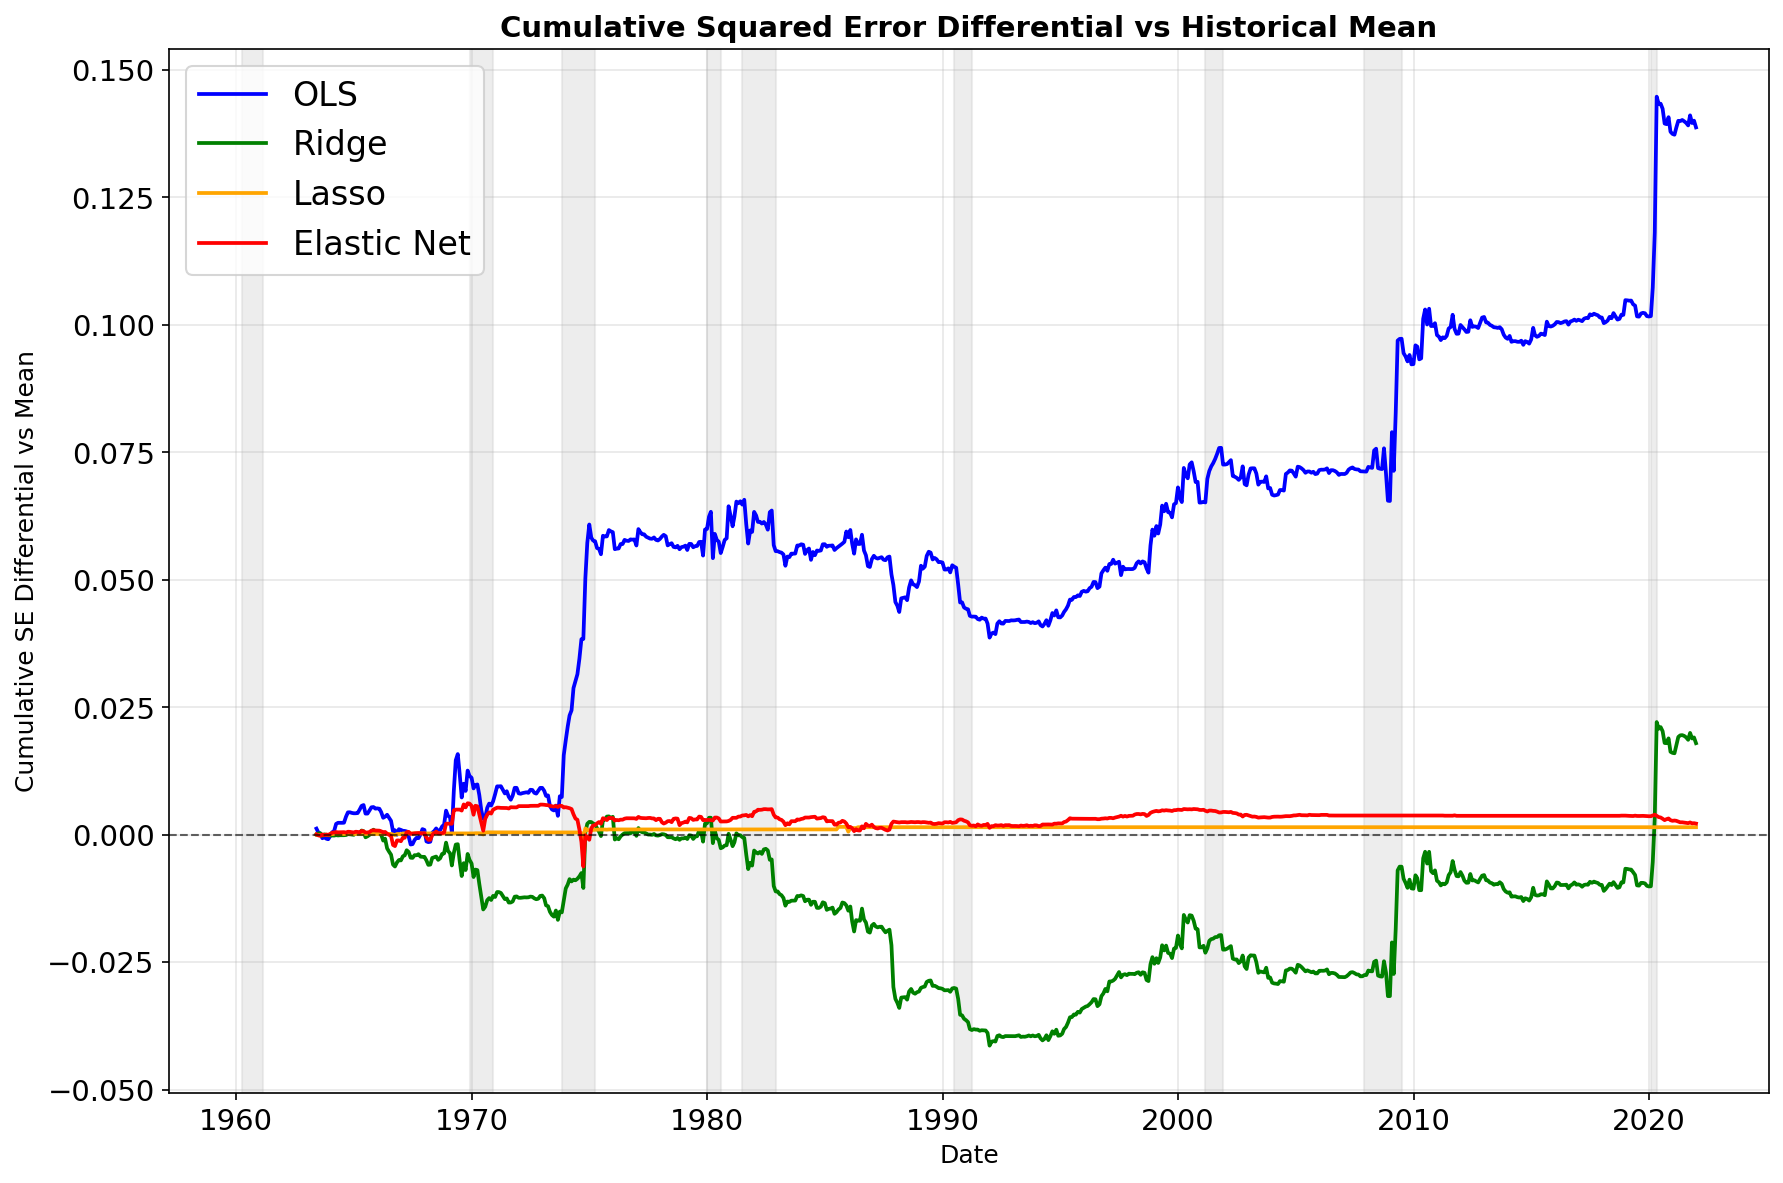
\includegraphics[width=0.8\textwidth]{Figures/cumulative_sse_differential.png}
  \end{center}
  
  \vspace{-0.8em}
  {\small
The chart shows the \textbf{cumulative Sum of Squared Error (SSE)} difference: $\sum_{t=1}^T [(y_t - \widehat{y}_t^{\text{model}})^2 - (y_t - \bar{y}_t)^2]$
  
  \begin{itemize}
    \item \highlight{Below zero} = model beats historical mean
    \item \highlight{Above zero} = model worse than historical mean
  \end{itemize}
  }
\end{frame}

\begin{frame}{Cumulative SSE Differential: What We Learn}
  \textbf{OLS (blue):}
  \begin{itemize}
    \item Starts well in 1970s, then \highlightred{catastrophically diverges}
    \item Post-2008: Accumulates 0.10+ in squared errors vs mean
    \item Problem: Extreme predictions amplify errors during crises
  \end{itemize}
  
  \vspace{0.5em}
  \textbf{Ridge (green):}
  \begin{itemize}
    \item \highlightgreen{Stays below zero throughout entire period}
    \item Occasionally beats mean (1980s-90s, 2020s)
    \item Most stable predictor -- never catastrophically wrong
  \end{itemize}
  
  \vspace{0.5em}
  \textbf{Lasso/Elastic Net (orange/red):}
  \begin{itemize}
    \item Track historical mean closely (near zero line)
    \item Slight improvement in the 2020s
    \item Conservative: avoid big losses but also miss opportunities
  \end{itemize}
  
  \vspace{0.5em}
  \textbf{Recessions (gray bars):} All models struggle, but Ridge degrades least
\end{frame}

\begin{frame}{Practical Lessons from Market Timing}

 \begin{block}{Why are all $R^2_{OS}$ negative?}
    \begin{itemize}
      \item Market returns are \highlight{extremely difficult to predict}
      \item Even small forecast errors are heavily penalized
      \item Historical mean is a surprisingly strong benchmark
      \item This is \highlight{typical} in equity premium prediction literature
    \end{itemize}
  \end{block}
  
  \vspace{1em}
  \textbf{What matters:}
  \begin{enumerate}
    \item \highlight{Relative performance:} Regularized models much closer to zero
    \item \highlight{Economic value:} Can poor $R^2$ still generate profits?
    \item \highlight{Directional accuracy:} Getting the sign right matters more than magnitude
  \end{enumerate}

\end{frame}


\begin{frame}{Sign Accuracy Analysis}
  \textbf{Getting the direction right is crucial for market timing:}
  
  \vspace{0.5em}
  \begin{table}[h]
    \centering
    \small
    \begin{tabular}{lccc}
      \toprule
      \textbf{Model} & \textbf{Sign Acc. (\%)} & \textbf{When Up (\%)} & \textbf{When Down (\%)} \\
      \midrule
      Historical Mean & 59.4 & 100.0 & 0.0 \\
      OLS & 57.8 & 68.7 & 42.0 \\
      Ridge & \highlightgreen{59.5} & 73.9 & 38.5 \\
      Lasso & 59.2 & 99.8 & 0.0 \\
      Elastic Net & 58.8 & 94.3 & 7.0 \\
      \bottomrule
    \end{tabular}
  \end{table}
  
  \vspace{0.5em}
  \textbf{Observations:}
  \begin{itemize}
    \item Ridge has \highlight{best overall sign accuracy} (59.5\%)
    \item Lasso/Elastic Net behaves like the historical mean (always bullish)
    \item OLS is more balanced but least accurate overall
    \item \highlight{Important:} 59.5\% accuracy can be economically valuable!
  \end{itemize}
\end{frame}

\begin{frame}{From Predictions to Portfolio Weights}
  \textbf{Market timing strategy:} Allocate between equity and risk-free asset
  
  \vspace{1em}
  \textbf{Mean-variance optimal weight:}
  \[
  \omega_t = \frac{1}{\gamma}\frac{\widehat{r}_{t+1}}{\widehat{\sigma}^2_t}
  \]
  where:
  \begin{itemize}
    \item $\widehat{r}_{t+1}$ = model's predicted excess return
    \item $\gamma = 5$ = risk aversion coefficient
    \item $\widehat{\sigma}^2_t$ = realized variance (rolling 60-month window)
    \item Constraints: $-1 \leq \omega_t \leq 1.5$ (allow 50\% leverage, 100\% cash)
  \end{itemize}
  
  \vspace{1em}
  \textbf{Portfolio return:}
  \[
  r_{t+1}^{\text{portfolio}} = \omega_t \cdot r_{t+1}^{\text{market}} + (1-\omega_t) \cdot r_f
  \]
\end{frame}

%----------------------------------------------------------------------------------------

\begin{frame}{Portfolio Weights Distribution}
  \begin{center}
    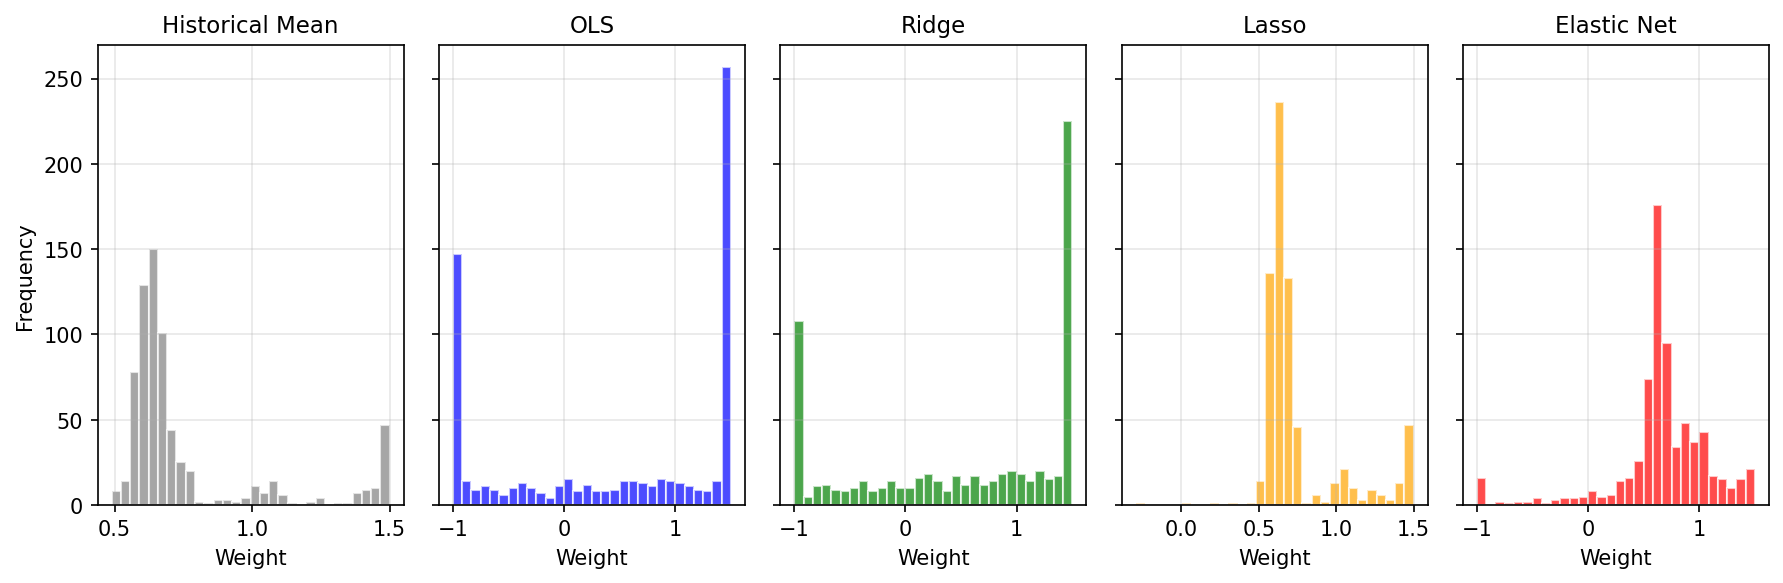
\includegraphics[width=1\textwidth]{Figures/portfolio_weights_distribution.png}
  \end{center}
  
%  \vspace{-0.8em}
\textbf{What are we looking at?} Histogram of equity weights over 672 months
\begin{itemize}
    \item OLS and Ridge weights often at constraints ($\omega = -1$ or $\omega = 1.5$)
    \item Lasso weights resembles the historical mean's: strong L1 penalty often zeros out most coefficients $\Rightarrow$ forecast $\approx$ mean
    \item E-net is between Lasso and Ridge, with weights more dispersed around 0.75
\end{itemize}

\end{frame}

\begin{frame}{Performance Metrics Summary}
  \textbf{Gross performance metrics:}\vspace{-0.1in}
  \begin{table}[h]
    \centering
  \renewcommand{\arraystretch}{1} % Increase space between rows
  \resizebox{\linewidth}{!}{\begin{tabular}{lccccc}
      \toprule
      \textbf{Strategy} & \textbf{Ann. Ret. (\%)} & \textbf{Sharpe} & \textbf{Max DD (\%)} & \textbf{Turnover} & \textbf{Win Rate (\%)} \\
      \midrule
      Buy \& Hold & 6.86 & 0.46 & -54.3 & 0.00 & --- \\
      \midrule
      Historical Mean & 4.32 & 0.39 & -50.8 & 0.13 & 42.0 \\
      OLS & 10.06 & 0.60 & -65.6 & \highlightred{7.77} & 54.8 \\
      Ridge & \highlightgreen{11.14} & \highlightgreen{0.70} & \highlightgreen{-51.0} & 6.34 & \highlightgreen{55.3} \\
      Lasso & 4.14 & 0.38 & -50.6 & 0.28 & 42.0 \\
      Elastic Net & 4.47 & 0.39 & -44.6 & 2.20 & 42.2 \\
      \bottomrule
    \end{tabular}}
  \end{table}
  
  \vspace{0.5em}
  \textbf{After 50 bps transaction costs for each rebalancing month:}
  \begin{table}[h]
    \centering
   \renewcommand{\arraystretch}{1} % Increase space between rows
  \resizebox{.6\linewidth}{!}{   \begin{tabular}{lcc}
      \toprule
      \textbf{Strategy} & \textbf{Ann. Ret. Net (\%)} & \textbf{Sharpe Net} \\
      \midrule
      Buy \& Hold & 6.86 & 0.46 \\
      OLS & 6.17 & 0.37 \\
      Ridge & \highlightgreen{7.97} & \highlightgreen{0.50} \\
      \bottomrule
    \end{tabular}}
  \end{table}
  
  \vspace{0.5em}
  \highlight{Takeaway:} Ridge achieves best risk-adjusted returns even after costs
\end{frame}


\begin{frame}{Cumulative Returns}
  \begin{center}
    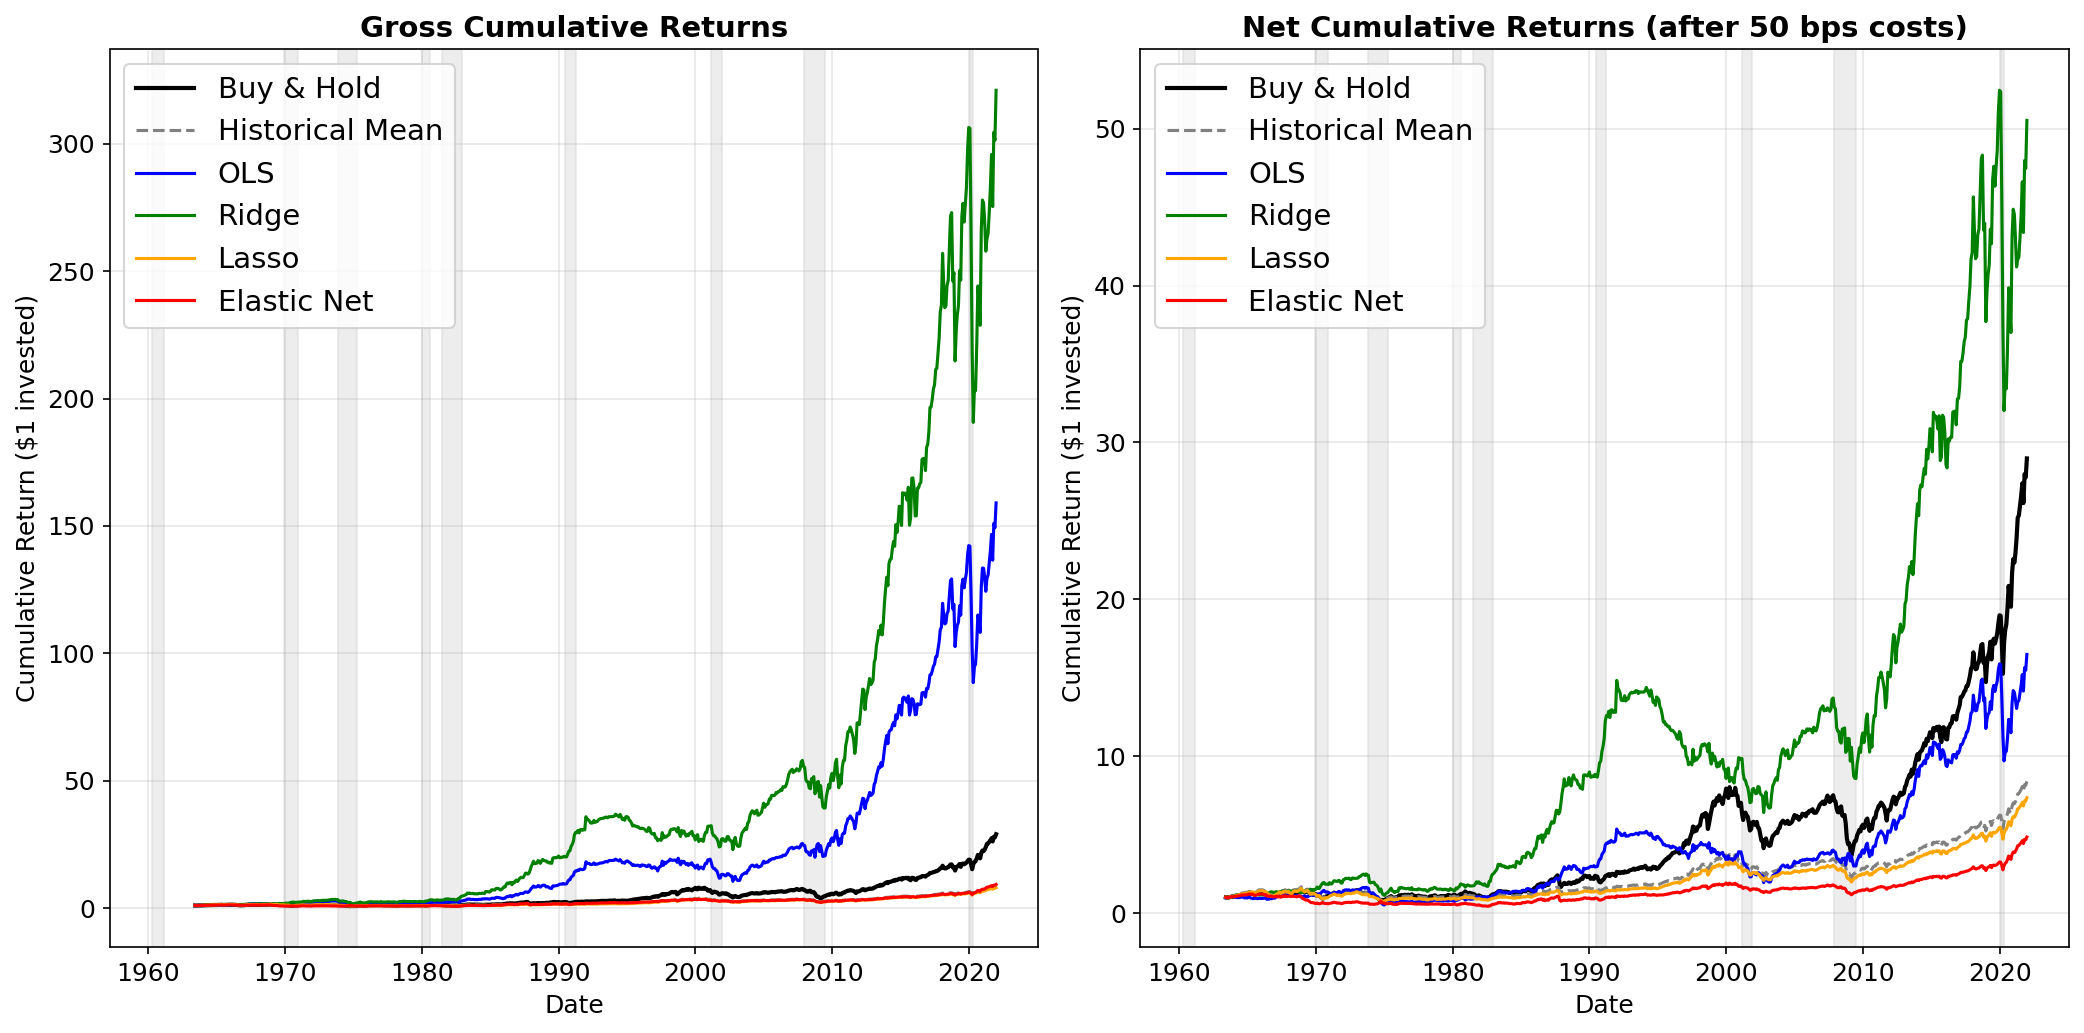
\includegraphics[width=1\textwidth]{Figures/market_timing_cumulative_returns.png}
  \end{center}
  
  \textbf{Left panel:} Gross returns (no transaction costs)\\ \textbf{Right panel:} Net returns (50 bps costs)
\end{frame}

\begin{frame}{Net Returns: Reality Check (Right Panel)}
  \textbf{After 50 bps (0.5\%) transaction costs per trade:}
  
  \vspace{0.5em}
  \textbf{OLS collapses:}
  \begin{itemize}
    \item \highlightred{\$158 $\rightarrow$ \$15} 
    \item High turnover (7.8$\times$ per year) $\Rightarrow$ costs destroy value
    \item \highlight{Lesson:} Overconfident predictions $\Rightarrow$ excessive trading
  \end{itemize}
  
  \vspace{0.5em}
  \textbf{Ridge survives:}
  \begin{itemize}
    \item \highlightgreen{\$320 $\rightarrow$ \$49} 
    \item Moderate turnover (6.3$\times$ per year) is still costly, but tolerable
    \item \highlightgreen{Still beats buy-and-hold after costs!}
  \end{itemize}
  
  \vspace{0.5em}
  \textbf{Historical Mean/Lasso/Elastic Net:}
  \begin{itemize}
    \item Largely unchanged (low turnover $<$ 2$\times$ per year)
    \item But still underperform buy-and-hold
  \end{itemize}
\end{frame}

\begin{frame}{Key Lessons for ML in Finance}
  
  \begin{enumerate}
    \item \textbf{Regularization is essential}
    \begin{itemize}
      \item OLS catastrophically overfits with many predictors (despite $p<<n$).
      \item Ridge provides the best balance: shrinkage without extreme sparsity
    \end{itemize}
    
    \vspace{0.5em}
    \item \textbf{Statistical vs economic performance diverge}
    \begin{itemize}
      \item Negative $R^2_{OS}$ does not mean no economic value
      \item 59.5\% directional accuracy $\Rightarrow$ 11\% annualized return
    \end{itemize}
    
    \vspace{0.5em}
    \item \textbf{Transaction costs matter enormously}
    \begin{itemize}
      \item High-turnover strategies (OLS) lose appeal after costs
      \item More stable predictions (Ridge) better preserve value
    \end{itemize}
    
    \vspace{0.5em}
    \item \textbf{Walk-forward testing is non-negotiable}
    \begin{itemize}
      \item In-sample $R^2$ would be misleading
      \item Real-time prediction reveals true model performance
    \end{itemize}
  \end{enumerate}
\end{frame}

\begin{frame}{Practical Implementation Considerations}
  
  \textbf{What we learned about deployment:}
  
  \vspace{0.5em}
  \begin{itemize}
    \item \textbf{Feature engineering:} Use lagged predictors to avoid look-ahead bias
    \begin{itemize}
      \item Predict $r_{t+1}$ using $X_t$ (known at time $t$)
      \item Easy to get wrong -- always validate timing!
    \end{itemize}
    
    \vspace{0.5em}
    \item \textbf{Hyperparameter tuning:} Use time-series cross-validation
    \begin{itemize}
      \item Never shuffle time series data
      \item Refit periodically as markets evolve
    \end{itemize}
    
    \vspace{0.5em}
    \item \textbf{Scaling:} Standardize features for regularized methods
    \begin{itemize}
      \item Ridge/Lasso/Elastic Net need consistent scales
      \item OLS is scale-invariant (no scaling needed)
    \end{itemize}
    
    \vspace{0.5em}
    \item \textbf{Constraints:} Impose realistic portfolio constraints
    \begin{itemize}
      \item Leverage limits, no-short-selling, etc.
      \item Unconstrained weights can be extreme and unrealistic
    \end{itemize}
  \end{itemize}
\end{frame}

%----------------------------------------------------------------------------------------
\section{Application 2: Factor Investing}
%----------------------------------------------------------------------------------------

\begin{frame}{A Different Question}

\textbf{Market timing:} \emph{When} to invest?
\begin{itemize}
  \item Predict aggregate market return
  \item Shift between stocks and bonds
\end{itemize}

\vspace{1em}
\textbf{Cross-sectional prediction:} \emph{Which stocks} to pick?
\begin{itemize}
  \item Predict relative performance across stocks
  \item Long winners, short losers
\end{itemize}

\vspace{1em}
\textbf{Key difference:}
\begin{itemize}
  \item Same methods, different data structure
  \item Cross-section: Much more data (many stocks)
  \item Often more successful than market timing
\end{itemize}

\end{frame}

%----------------------------------------------------------------------------------------

\begin{frame}{The Factor Investing Framework}

\textbf{Traditional approach:}
\begin{enumerate}
  \item Identify a characteristic (e.g., book-to-market)
  \item Rank stocks by that characteristic
  \item Long high-ranked stocks, short low-ranked
  \item Earn the ``factor premium''
\end{enumerate}

\vspace{1em}
\textbf{Examples:}
\begin{itemize}
  \item Value: High book-to-market outperforms
  \item Momentum: Past winners continue to win
  \item Size: Small stocks outperform (historically)
  \item Profitability: Profitable firms outperform
\end{itemize}

\vspace{1em}
\textbf{Question:} Which characteristics? How to combine them?

\end{frame}

%----------------------------------------------------------------------------------------

\begin{frame}{Data Structure: Panel}
\textbf{Cross-sectional regression:}
\[
r_{i,t+1} = x_{i,t}'\boldsymbol{\beta} + \epsilon_{i,t+1}
\]

\vspace{0.5em}
\textbf{Interpretation:}
\begin{itemize}
  \item Characteristics $x_{i,t}$ predict returns at $t+1$
  \item $\beta_j$: Premium associated with characteristic $j$
  \item Linear combination of characteristics $\Rightarrow$ expected return
\end{itemize}

\vspace{0.5em}
\textbf{Panel structure:} Observations are stock-months.
\begin{itemize}
  \item Many more observations ($N \times T$ vs.\ $T$)
  \item More power to detect patterns (number of stocks $N$ can be large)
\end{itemize}

\vspace{1em}
\textbf{Challenge:}
\begin{itemize}
  \item Many candidate characteristics ($p$ large)
  \item Characteristics are correlated
  \item Which ones really matter?
\end{itemize}

\end{frame}

%----------------------------------------------------------------------------------------

\begin{frame}{The ``Zoo'' of Characteristics}

\textbf{Harvey, Liu \& Zhu (2016):}
\begin{itemize}
  \item 300+ factors published in academic journals
  \item Most discovered through data mining
  \item Many are likely spurious
\end{itemize}

\vspace{1em}
\textbf{Gu, Kelly \& Xiu (2020):}
\begin{itemize}
  \item 900+ firm characteristics
  \item Comprehensive dataset for ML
\end{itemize}

\vspace{1em}
\textbf{Problem:}
\begin{itemize}
  \item Too many predictors for OLS
  \item Many are correlated (size, value, profitability overlap)
  \item Need principled way to select/combine
\end{itemize}

\end{frame}

%----------------------------------------------------------------------------------------

\begin{frame}{Kozak, Nagel \& Santosh (2020): Key Insight}

\textbf{Traditional approach:}
\begin{itemize}
  \item Select a small number of characteristics
  \item Justify selection with theory or prior evidence
  \item Problem: Which ones? Selection is arbitrary.
\end{itemize}

\vspace{1em}
\textbf{Kozak, Nagel \& Santosh (KNS) approach:}
\begin{itemize}
  \item Use \emph{all} $100+$ characteristics
  \item Apply Ridge regression to handle high dimensionality
  \item Let shrinkage determine relative importance
\end{itemize}

\vspace{1em}
\textbf{Key insight:} Ridge shrinkage is equivalent to imposing a \highlight{prior belief} that most characteristics have small effects.

\end{frame}

%----------------------------------------------------------------------------------------

%----------------------------------------------------------------------------------------


%----------------------------------------------------------------------------------------

\begin{frame}{From Predictions to Portfolios}

\textbf{Procedure:}
\begin{enumerate}
  \item Estimate $\widehat{\beta}$ using data up to month $t$
  
  \vspace{0.3em}
  \item For each stock $i$, compute predicted return:
  \[
  \widehat{r}_{i,t+1} = x_{i,t}'\widehat{\boldsymbol{\beta}}
  \]
  
  \vspace{0.3em}
  \item Rank stocks by $\widehat{r}_{i,t+1}$
  
  \vspace{0.3em}
  \item Form portfolio:
  \begin{itemize}
    \item Long: Top decile (highest predicted returns)
    \item Short: Bottom decile (lowest predicted returns)
  \end{itemize}
  
  \vspace{0.3em}
  \item Observe realized portfolio return in month $t+1$
  
  \vspace{0.3em}
  \item Roll forward, repeat
\end{enumerate}

\end{frame}

%----------------------------------------------------------------------------------------

\begin{frame}{Walk-Forward Backtesting}

\begin{center}
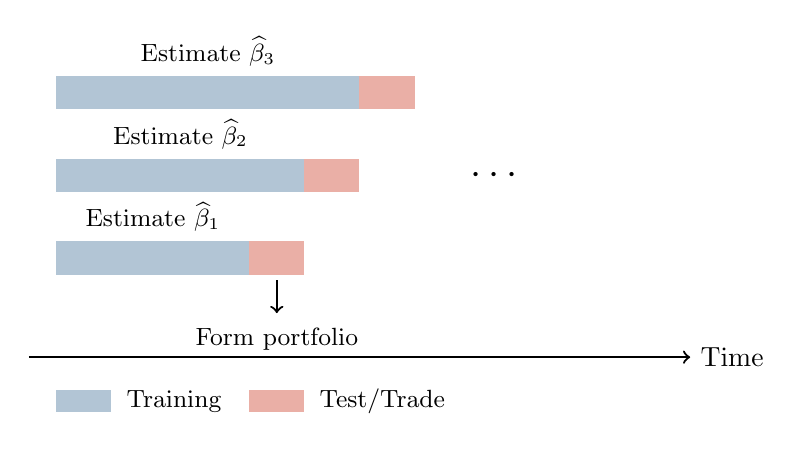
\begin{tikzpicture}[scale=0.7]
  % Timeline
  \draw[thick, ->] (0, 0) -- (12, 0) node[right] {Time};
  
  % Estimation period 1
  \fill[ThemeBlue, opacity=0.3] (0.5, 1.5) rectangle (4, 2.1);
  \node[above] at (2.25, 2.1) {\small Estimate $\widehat{\beta}_1$};
  
  % Predict period 1
  \fill[AccentOrange, opacity=0.5] (4, 1.5) rectangle (5, 2.1);
  
  % Arrow
  \draw[->, thick] (4.5, 1.4) -- (4.5, 0.8);
  \node[below] at (4.5, 0.7) {\small Form portfolio};
  
  % Estimation period 2
  \fill[ThemeBlue, opacity=0.3] (0.5, 3) rectangle (5, 3.6);
  \node[above] at (2.75, 3.6) {\small Estimate $\widehat{\beta}_2$};
  
  % Predict period 2
  \fill[AccentOrange, opacity=0.5] (5, 3) rectangle (6, 3.6);
  
  % Estimation period 3
  \fill[ThemeBlue, opacity=0.3] (0.5, 4.5) rectangle (6, 5.1);
  \node[above] at (3.25, 5.1) {\small Estimate $\widehat{\beta}_3$};
  
  % Predict period 3
  \fill[AccentOrange, opacity=0.5] (6, 4.5) rectangle (7, 5.1);
  
  % Dots
  \node at (8.5, 3.3) {\Large $\cdots$};
  
  % Legend
  \fill[ThemeBlue, opacity=0.3] (0.5, -1) rectangle (1.5, -0.6);
  \node[right] at (1.6, -0.8) {\small Training};
  \fill[AccentOrange, opacity=0.5] (4, -1) rectangle (5, -0.6);
  \node[right] at (5.1, -0.8) {\small Test/Trade};
\end{tikzpicture}
\end{center}

\vspace{0.5em}
Re-estimate periodically (monthly or quarterly).\\ 
Track cumulative returns.

\end{frame}

%----------------------------------------------------------------------------------------

\begin{frame}{Results: Shrinkage Helps Substantially}

\textbf{Kozak, Nagel \& Santosh (2020) findings:}

\vspace{1em}
\begin{itemize}
  \item Ridge substantially outperforms OLS out-of-sample
  
  \vspace{0.5em}
  \item Optimal $\lambda$ implies significant shrinkage
  \begin{itemize}
    \item Data supports skepticism about many characteristics
  \end{itemize}
  
  \vspace{0.5em}
  \item Long-short portfolios achieve Sharpe ratios $> 1$
  
  \vspace{0.5em}
  \item Results robust across different sample periods
  
  \vspace{0.5em}
  \item Better performance than selecting ad-hoc subsets
\end{itemize}

\vspace{1em}
\textbf{Key message:} Regularization is not just a technical fix --- it embodies economically sensible skepticism.

\end{frame}

\begin{frame}{Lessons from KNS (2020) for Practitioners}
  
  \begin{enumerate}
    \item \highlight{Do not search for the ``true'' sparse model}
    \begin{itemize}
      \item Financial markets are complex; many factors matter
      \item Embrace high-dimensional methods rather than fight dimensionality
    \end{itemize}
    
    \vspace{0.5em}
    \item \textbf{Consider Ridge as baseline regularization method}
    \begin{itemize}
      \item Especially when predictors are correlated (common in finance)
      \item More robust than Lasso or OLS
      \item Can always add L$_1$ penalty if you need interpretability
    \end{itemize}
        
    \vspace{0.5em}
    \item \highlight{Always validate out-of-sample}
    \begin{itemize}
      \item In-sample fit is misleading with many predictors
      \item Use proper time-series validation (walk-forward, cross-validation)
      \item Test economic value, not just statistical fit
    \end{itemize}
  \end{enumerate}
\end{frame}

%----------------------------------------------------------------------------------------

%----------------------------------------------------------------------------------------

\begin{frame}{Some Key Practical Considerations}

\textbf{1. \highlightred{Transaction costs}}
\begin{itemize}
  \item ML strategies can have high turnover
  \item Trading costs erode returns
  \item May need to constrain turnover
\end{itemize}

\vspace{0.5em}
\textbf{2. \highlightred{Capacity constraints}}
\begin{itemize}
  \item ML strategies tend to work best in small/mid caps
  \item Large trades move prices (market impact)
  \item May not scale to institutional size (liquidity matters)
\end{itemize}

\vspace{0.5em}
\textbf{3. Data quality}
\begin{itemize}
  \item Point-in-time data essential (avoid look-ahead)
  \item Survivorship bias: Include delisted firms
  \item Data errors can drive spurious results
\end{itemize}

\end{frame}

%----------------------------------------------------------------------------------------
%----------------------------------------------------------------------------------------


%----------------------------------------------------------------------------------------
\section{Summary and Next Steps}
%----------------------------------------------------------------------------------------

\begin{frame}{Key Takeaways from Today}
  \begin{enumerate}
    \item Market timing is very difficult with linear models --- even regularization often helps only modestly
    \begin{itemize}
    \item Monthly return volatility $\approx 4$--$5\%$
    \item Predictable component $\approx 0.5\%$ (if any)
    \item Signal buried in noise
\item The relationship between ERP and the state of the economy might be non-linear
    \end{itemize}
    \vspace{0.3em}
    \item Cross-sectional prediction benefits more clearly from shrinkage
  \begin{itemize}
  \item Shrinkage = Skepticism about predictability 
  \item Economically sensible assumption given market timing evidence
  \end{itemize}
    \vspace{0.3em}
    \item Always evaluate the economic benefit of your model above and beyond statistical accuracy
 \end{enumerate}
\end{frame}


\begin{frame}{Readings and Next Steps}
  \textbf{Readings for Today's Lecture:}
  \begin{itemize}
    \item Goyal, Welch, \& Zafirov (2024). ``A comprehensive 2022 look at the empirical performance of equity premium prediction." \emph{The Review of Financial Studies}.\hfill \textit{[Recomm.]}
    \item Kozak, Nagel \& Santosh (2020), ``Shrinking the Cross-Section,'' \emph{Journal of Financial Economics}\hfill \textit{[Supp.]}
  \end{itemize}
  \vspace{1em}
  
  \textbf{Topics for the next lecture:}

\vspace{1em}
\begin{itemize}
  \item Tree-based methods and ensemble learning
\begin{itemize}
  \item Random Forests: Bagging + feature sampling
  \item Gradient Boosting: XGBoost, LightGBM
  \item Non-linear relationships and interactions
\end{itemize}
\item Key advantage: Automatically capture non-linearities and interactions that linear models miss.

\item Can trees resurrect market timing and time-series predictability? 
\end{itemize}
  \end{frame}

\begin{frame}[plain]
  \centering
  \vfill
  {\Large Questions?}
  \vfill
\end{frame}



%----------------------------------------------------------------------------------------

%----------------------------------------------------------------------------------------


%----------------------------------------------------------------------------------------


\end{document}